%!TEX root = ../thesis_a4.tex

\chapter[A new perspective: ontology-based tag recommendation][A new pers.: ontology-based tag rec.]{A new perspective: ontology-based tag recommendation}
\label{sec:ontology}

\section{Introduction}
\label{sec:ontology:introduction}
%It is important to clarify that the focus of our exploratory research is not that much in the design and definition of the ontology, as its application in a tag recommendation system.

In this chapter we present a new perspective on tag recommendation systems and explore how can it tackle some of the tagging issues that have been identified in the previous chapters. 
The goal is to design a tag recommendation system that further improves the quality of resource annotations. 
In particular, the recommendation system is focused on helping users to generate more comprehensive, coherent and semantically meaningful resource annotations.
%For this purpose, we incorporate several ideas proposed by different authors in the tagging literature. 

A particularity of the folksonomies emerging from tagging systems is that tags are organised in a flat hierarchy, typically detached from a uniquely identifiable semantic meaning~\citep{golder2006,halpin2006}. Hence, tags are not restricted to a predefined set of concepts or a fixed vocabulary.
We have seen that this has the advantage of enabling a certain flexibility and ease of use from the users' point of view (Sec.~\ref{sec:SOA:tagging_systems}).
This is one of the reasons why  tagging systems have succeeded as a popular organisation system in online sharing platforms~\citep{shirky2005ontology,halpin2006,Cattuto2006}. 
However, we have also seen that this approach presents some disadvantages because different tagging conventions may coexist in a single folksonomy, and because the semantic meaning of tags can not be unambiguously determined (Sec.~\ref{soa:tagging_problems}).

The flexibility of user-generated folksonomies is often opposed to the accurateness and rigidity of \emph{ontologies}, which are designed by domain experts.
Ontologies provide, for a given domain, an unambiguous formalisation of its concepts, entities and their relations. 
Hence, where folksonomies feature free-form textual labels with no predefined semantic meaning, ontologies feature detailed concept hierarchies interlinked with semantically meaningful relations.
%These concepts are defined as a hierarchy of classes in the ontology, with object properties that define possible relations between instances (or individuals) of these classes.

Although folksonomies and ontologies appear to be opposed ways in which knowledge can be represented, some authors suggest that these are, in fact, complementary approaches that can be combined. %~\citep{Mika2007a}. 
For instance, some authors propose techniques for analysing folksonomies and automatically generating tag hierarchies or identifying simple semantic relations between tags~\citep{Merholz2004,halpin2006,Heymann2006a,Mika2007a,Hwang2007}. These automatically derived hierarchies and semantic relations can be used to aid ontology creation processes.
Other authors propose to enhance the semantic value of folksonomies by establishing unambiguous relations between tags and concepts defined in an ontology~\citep{Good2007,Passant2007a}.
Similarly, other authors suggest to model folksonomies through the use of ontologies, enabling the inclusion of semantically structured content in folksonomies. In this direction, several \emph{tagging ontologies} have been proposed which conceptualise the different agents involved in a tagging process~\citep{Newman2005,Limpens2007,Echarte2007,Passant2008a,Kim2010,Ding2010a}.
The use of tagging ontologies allows the definition of semantic relations between tags that can be used, for example, to tackle synonymy and ambiguity problems. Furthermore, tagging ontologies allow the interoperability of folksonomies among different sharing platforms by unifying the way in which tagging information is modelled.
%In this chapter, we explore an approach of tag recommendation which is based on the use of a tagging ontology extended.
A comprehensive literature review of works combining folksonomies and ontologies can be found in~\cite{limpens2009linking}.

In this chapter, we explore the idea of combining folkosnomies and ontologies to improve the tag recommendation system described in the previous chapters.
For this purpose, we define an ontology which extends a previously existing tagging ontology (see below).
The ontology that we use, besides formalising tagging concepts, allows the categorisation of tags and resources into semantically meaningful categories.
More specifically, it can categorise tags into a number of information facets which are particularly relevant in the audio domain. 
For example, the ontology specifies that tags like \atag{guitar} and \atag{violin} annotate musical instruments, and that tags like \atag{english} or \atag{german} describe the spoken language of a sound. 
Furthermore, the ontology defines a number of broad audio categories and relates them to the aforementioned tag categories. In this way, we are able to specify which information facets are relevant for every audio category. Following the previous example, the ontology can specify that tags describing musical instruments are typically relevant for music recordings, while tags indicating a spoken language are most relevant for voice recordings.
Taking advantage of this knowledge, we propose an ontology-based tag recommendation system that is able to implement two features which clearly distinguish it from previous approaches. 
On the one hand, tags recommended by the system are not presented to users as a single list of suggestions, but grouped into the different information facets defined by tag categories in the ontology. 
On the other hand, the system can predict which information facets are relevant for a given sound, and then suggest users to add tags that cover these facets. In this way, the tag recommendation system assists users not only by recommending tags, but also by helping them in choosing which kind of information is relevant for describing a particular sound.

Little research has been carried out on using ontologies to drive tag recommendation systems, and the followed approaches are conceptually different from the one we take here.
In the works by~\cite{Adrian2007} and~\cite{Prokofyev2012}, a tag recommendation system is described for textual resources in which natural language processing techniques are used to identify relevant keywords in a resource. Then, these keywords are matched against ontology concepts of external knowledge bases to retrieve other related concepts to be presented as tag recommendations. Hence, in these cases, the ontologies are not used to guide the recommendation process nor embed domain-specific knowledge relevant for the annotation process.
\cite{Guy2006} introduced an idea which is similar to that of guiding the recommendation process. In particular, they suggested that tagging can be improved by ``providing users with a set of helpful heuristics that promote good tag selection, such as a checklist of questions that could be applied to the object being tagged, in order to direct the tagger to various salient characteristics'', but no further research was carried out.
\cite{Chen2008a}, describe a tag recommendation system for images in which tags are presented to users organised in a number of predefined categories. The categories defined by~\cite{Chen2008a} are, in fact, resource categories which group images into broad categories such as ``portrait'', ``animal'' or ``architecture''. Given an image to annotate, the recommendation system can estimate the most relevant categories by computing content-based similarity measures with already categorised images in a ground truth. Then, the system can recommend the most popular tags for each of the estimated relevant categories.
Conversely, our approach is focused on taking advantage of the combination of tag categories and resources categories, and makes use of an ontology that formalises these categories and that allows us establish further semantic relations.

The interface of the ontology-based tag recommendation system described in this chapter allows users to introduce tags in an ``attribute:value'' fashion, in which the ``attribute'' represents a tag category and the ``value'' is the actual tag\footnote{To clarify further explanations, we will refer to those tags that are introduced with a tag category as \emph{attribute-tags}.}. For example, an hypothetical attribute-tag like \atag{instrument:guitar} has the attribute ``instrument'' and the value ``guitar''. The attribute clarifies the semantic context of the actual tag, specifying in this case that ``guitar'' is an ``instrument''.
Users can select a tag category, and then the system provides specific tag recommendations tailored to that category. However, besides choosing tags from the list of recommendations, users can also type their own, therefore creating new tags for a given tag category. 
In this way, users are able to contextualise tags in a particular tag category, making their semantic meaning more explicit.
In a sense, the concept of tag categories included in the tag recommendation system is extended to the whole tagging interface. 
Tag categories are therefore not only useful to guide the annotation process and provide tag recommendations, but also to allow the introduction of tags with less ambiguous semantic meaning by explicitly indicating their semantic facets~\citep{halpin2006}.
%- Also proposed in \cite{Toderici2010}, learn relations between tags and video features, mine web pages to derive categories common to the tags, then predict categories for new uploads (work with 9000 categories, not designed by experts nor thought as a simple thing for users) - YOUTUBE
This is similar to the idea of \emph{triple-tags} introduced by~\cite{Catt2006}, which was later used in the Flickr API\footnote{\url{http://www.flickr.com/groups/api/discuss/72157594497877875/}} under the name of \emph{machine-tags}. Triple-tags are normal tags formatted with a specific syntax that allows the precise specification of the meaning of a tag. By using a syntax such as ``namespace:attribute=value'', tags can be used, for example, to precisely specify geolocations (e.g.,~\{\atag{geo:lat=53.1234}, \atag{geo:long=-2.5678}\}). Hence, as far as tags contain a known namespace and attribute, their meaning can be easily interpreted. Using triple-tags, the Flickr API can respond to complex queries that operate on the namespace, attribute and value of the tags.
However, to our knowledge, triple-tags can only be used through the Flickr API, and no user interfaces nor recommendation systems have been developed for them.

To evaluate the tag recommendation system described here, we perform an online experiment with more than 200 participants. We then compare the ontology-based tag recommendation system with our previous class-based recommendation system described in Chapter~\ref{sec:class}. In this online experiment, a group of participants annotate a pool of sounds using the ontology-based system, while another group annotate the same sounds using the class-based system. Then, we define a number of metrics (some of them already used in the previous chapters) to compare both systems. Furthermore, to complement the results of that experiment, we perform a second experiment in which the ontology-based interface is deployed in Freesound. With this second experiment, we collect real-world data usage of the interface that we analyse and compare with the results from the first experiment. In general, our results show that the ontology-based tag recommendation system can effectively help in improving sound annotations in those cases where users spend enough time and give enough importance to the annotation process.

The rest of the chapter is organised as follows. First, we describe in detail the ontology-based tag recommendation system, including the design and population of its ontology, and the user interface (Sec.~\ref{sec:ontology:method}). Then, we describe the online experiments and metrics that we used to evaluate the system (Sec.~\ref{sec:ontology:evaluation_method}). Evaluation results are reported in Sec.~\ref{sec:ontology:results}, and the chapter ends with a discussion about our findings  (Sec.~\ref{sec:ontology:conclusion}).


\section{Method}
\label{sec:ontology:method}
\subsection{Ontology design}
\label{sec:ontology:design}
The ontology that we use to drive our tag recommendation system is an extension of the Modular Unified Tagging Ontology, or MUTO\footnote{MUTO: Modular Unified Tagging Ontology. \url{http://muto.socialtagging.org/core/v1.html}.} for short~\citep{Lohmann2011}.
The MUTO ontology builds on top of previously existing tagging ontologies, and it was originally proposed to unify them. 
For this reason, we use it as a starting point for our ontology. 
In the core of the MUTO ontology, the \atag{muto:Tagging} class is defined along with several object properties\footnote{In ontologies, object properties are used to relate instances (individuals) of particular classes. For example, using object properties it can be specified that a particular instance of a class \texttt{:ClassA}, is \texttt{:similarTo} an instance of \texttt{:ClassB}. In that case, \texttt{:similarTo} is an object property with a particular semantic meaning that must be defined in the ontology. Object properties can impose restrictions on the types of instances that can be related (i.e.,~on the class of instances). This is done by defining a \emph{domain} and \emph{range} for an object property.} to indicate, among others, a resource that is tagged (\atag{muto:hasResource} of type \atag{rdfs:Resource}), the tag assigned to the resource (\atag{muto:hasTag} of type \atag{muto:Tag}), and the user that made the tag assignment (\atag{muto:hasCreator} of type \atag{sioc:UserAccount}). Particular users, tags and resources are modelled as instances of the classes \atag{sioc:UserAccount}, \atag{muto:Tag} and \atag{rdfs:Resource} respectively.
Using such an ontology, it is possible to model the contents of a folksonomy in a structured manner.
However, the MUTO ontology (together with the other existing tagging ontologies) is focused on the representation of the tagging process, but does not a priori incorporate other kinds of knowledge which may be specific to the particular domain of a tagging system.
To overcome that limitation, we propose a simple extension of the MUTO ontology which meets the requirements of our ontology-based tag recommendation system. 

We extend the tagging ontology in several ways. First, we add a number of subclasses to the \atag{muto:Tag} class.
These subclasses are used instead of~\atag{muto:Tag}, and therefore the tags in our ontology are modelled as instances of these subclasses (right side of Fig.~\ref{fig:ontology_concept}).
In our ontology, \atag{muto:Tag} subclasses conceptualise a number of tag categories according to different kinds of information facets conveyed by tags. 
Hence, a tag category groups a set of tags that share some semantic meaning in the audio domain.
For example, we define tag categories\footnote{Similarly to the audio classes introduced in Chapter~\ref{sec:class}, to refer to tag classes we may use the terms ``class'' or ``category'' indistinctly.} such as \atag{fso:InstrumentTag} or \atag{fso:MicrophoneTag}, which include tags that convey information about the musical instruments present in a recoding, or about the microphones that were used\footnote{In this chapter we use the prefix \texttt{fso:} to denote the classes and other definitions of our ontology. The prefix \texttt{fso:} stands for ``Freesound ontology''. However, this is just a convenient name we use to make our explanations more clear.}.
A complete list of the different tag categories defined in the ontology is given in Table~\ref{tab:ontology_tag_categories}. 
More details on the definition of tag categories and on how we populate them with tag instances are given in Sec.~\ref{sec:ontology:population}.

\begin{figure}[t]
  \centering
  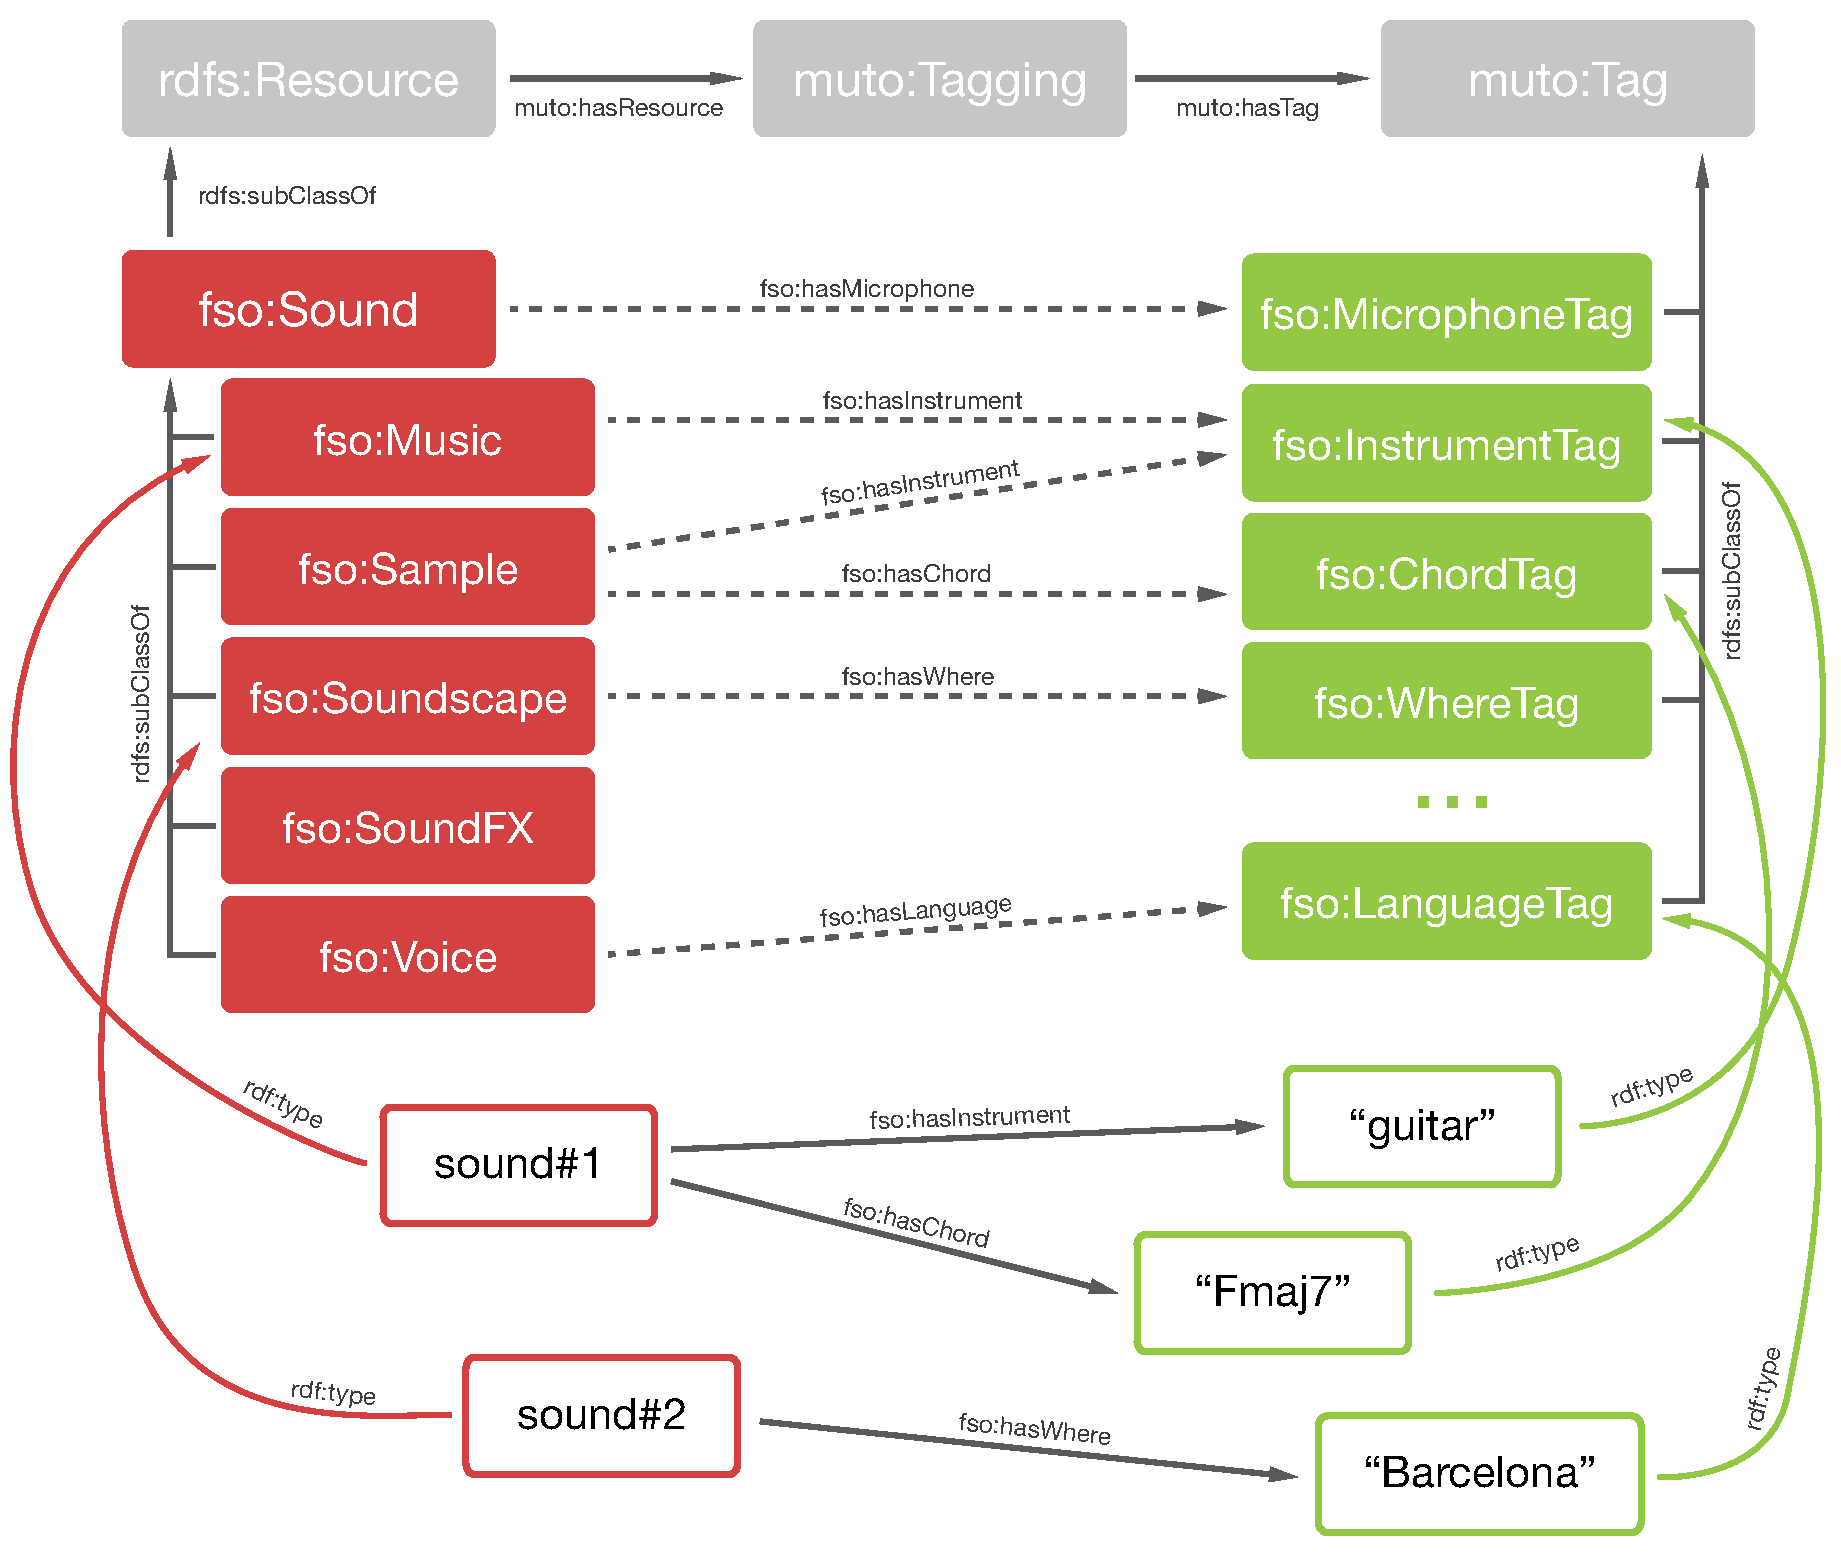
\includegraphics[width=1.0\textwidth]{ch06_ontology/pics/diagram_ontology_model}
  \caption[Conceptual diagram of the extension of the MUTO ontology]{Conceptual diagram of the extension of the MUTO ontology that drives the tag recommendation system. Solid boxes represent the classes of the ontology, while arrows indicate object properties. Dashed arrows represent the definitions of the object properties that relate audio categories with tag categories. The boxes at the bottom exemplify tag and resource instances. For the sake of clarity, only a small subset of \texttt{muto:Tag} subclasses are displayed in this figure. A complete list can be found in Table~\ref{tab:ontology_tag_categories}.}
  \label{fig:ontology_concept}
\end{figure}


Following the same idea of tag categories, we also extend the MUTO ontology by incorporating \atag{rdfs:Resource} subclasses that allow the grouping of resources into a number of audio categories (left side of Fig.~\ref{fig:ontology_concept}). 
%In the specific use case of our tag recommendation system, and given that we recommend tags for sounds, 
We define a generic \atag{fso:Sound} subclass for \atag{rdfs:Resource}, and five subclasses for the \atag{fso:Sound} class which correspond to the audio classes that we have already defined in our previous version of the tag recommendation system (Sec~\ref{class:sec:classification_system}). 
As it can be seen in Fig.~\ref{fig:ontology_concept}, the five subclasses of \atag{fso:Sound} are named in accordance with their corresponding audio class names.%\footnote{
%\texttt{fso:SoundFX} for \textsc{SoundFX}, 
%\texttt{fso:Soundscape} for \textsc{Soundscape}, 
%\texttt{fso:Sample} for \textsc{Sample}, 
%\texttt{fso:Music} for \textsc{Music} and 
%\texttt{fso:Voice} for \textsc{Voice}.}.

Finally, we also extend the tagging ontology by defining a number semantic relations in the form of object properties.
The purpose of these object properties is to represent relations between tag and resource instances (dashed lines in Fig.~\ref{fig:ontology_concept}).
Every included object property defines, as its range, a particular \atag{muto:Tag} subclass, and as its domain, at least one of the \atag{rdfs:Resource} subclasses. Therefore, we define as many object properties as tag categories. These object properties are named according to their ranged tag category. 
For example, the property \atag{fso:hasInstrument} ranges instances of \atag{fso:InstrumentTag}, and its domain includes instances of \atag{fso:Sample} and \atag{fso:Music} audio categories.
Therefore, \atag{fso:hasInstrument} can relate sounds belonging to either the \atag{fso:Sample} or \atag{fso:Music} classes, with tag instances of the type \atag{fso:Ins\-tru\-ment\-Tag}.
By inspecting the domains and ranges of these object properties, our ontology can determine which tag categories are relevant when describing a resource of a given audio category. 
For instance, and following the previous example, the ontology can determine that \atag{fso:InstrumentTag} tags, are relevant when annotating sounds of the \atag{fso:Music} or \atag{fso:Sample} audio categories, but that are not so relevant when annotating sounds of other categories such as \atag{fso:Soundscape}.
Object properties can be defined with multiple domains, meaning that a particular tag category can be considered relevant to more than one audio category.
In Table~\ref{tab:ontology_tag_categories} we show, for every tag category, its corresponding object property range, name and domain.

\begin{sidewaystable}
\ra{1.1}
\tiny
\begin{center}
\footnotesize
\begin{tabular}{@{}p{3.4cm}lp{4.6cm}l@{}}
\toprule
\textbf{Tag category/Object property range} & \textbf{Object property name} & \textbf{Object property domain} & \textbf{Information facet description} \\ 
\midrule 
\texttt{fso:ActionTag} & \texttt{fso:hasAction} & \texttt{fso:SoundFX}, \texttt{fso:Soundscape} & Physical activities captured in the recording \\
\texttt{fso:AgeTag} & \texttt{fso:hasAge} & \texttt{fso:Voice} & Age of the speaker or speakers \\
\texttt{fso:ArticulationTag} & \texttt{fso:hasArticulation} & \texttt{fso:Music}, \texttt{fso:Sample} & Performance or playing technique \\
\texttt{fso:ChordTag} & \texttt{fso:hasChord} & \texttt{fso:Music} & Music chords present in the recording \\
\texttt{fso:DynamicsTag} & \texttt{fso:hasDynamics} & \texttt{fso:Music}, \texttt{fso:Sample} & General loudness characteristics \\
\texttt{fso:EnvelopeTag} & \texttt{fso:hasEnvelope} & \texttt{fso:Sample} & Envelope of a sound at the note level \\
\texttt{fso:GearTag} & \texttt{fso:hasGear} & \texttt{fso:Sound} & Gear used to generate the sound \\
\texttt{fso:GenderTag} & \texttt{fso:hasGender} & \texttt{fso:Voice} & Gender of the speaker or speakers \\
\texttt{fso:GenreTag} & \texttt{fso:hasGenre} & \texttt{fso:Music}, \texttt{fso:Sample} & Music genre \\
\texttt{fso:InstrumentTag} & \texttt{fso:hasInstrument} & \texttt{fso:Music}, \texttt{fso:Sample} & Instrument names, brands or types \\
\texttt{fso:KeyTag} & \texttt{fso:hasKey} & \texttt{fso:Music} &  Music tonality of the recording  \\
\texttt{fso:LanguageTag} & \texttt{fso:hasLanguage} & \texttt{fso:Voice} & Languages present in the sound \\
\texttt{fso:MaterialTag} & \texttt{fso:hasMaterial} & \texttt{fso:SoundFX} & Material of sound sources present in the recording \\
\texttt{fso:MeterTag} & \texttt{fso:hasMeter} & \texttt{fso:Music} &  Music time signature information \\
\texttt{fso:MicrophoneTag} & \texttt{fso:hasMicrophone} & \texttt{fso:Sound} & Microphone names, brands and types \\
\texttt{fso:MoodTag} & \texttt{fso:hasMood} & \texttt{fso:Sound} & Moods and emotions conveyed by the sound \\
\texttt{fso:NoteTag} & \texttt{fso:hasNote} & \texttt{fso:Sample} & Music note present in the recording \\
\texttt{fso:OnomatopeiaTag} & \texttt{fso:hasOnomatopeia} & \texttt{fso:SoundFX} & Phonetic imitations of the sound \\
\texttt{fso:ProcessingTag} & \texttt{fso:hasProcessing} & \texttt{fso:Sound} & Techniques used to process the recording \\
\texttt{fso:RecordingTag} & \texttt{fso:hasRecording} & \texttt{fso:Sound} & Recording techniques used to produce the sound \\
\texttt{fso:SoftwareTag} & \texttt{fso:hasSoftware} & \texttt{fso:Sound} & Software names, brands or types \\
\texttt{fso:TempoTag} & \texttt{fso:hasTempo} & \texttt{fso:Music} & Tempo information \\
\texttt{fso:TypeTag} & \texttt{fso:hasType} & \texttt{fso:Sound} & Generic classification of a sound \\
\texttt{fso:WhatTag} & \texttt{fso:hasWhat} & \texttt{fso:SoundFX}, \texttt{fso:Soundscape} & Sound sources present in the recording \\
\texttt{fso:WhenTag} & \texttt{fso:hasWhen} & \texttt{fso:Soundscape} & Indication of the moment when the sound was recorded  \\
\texttt{fso:WhereTag} & \texttt{fso:hasWhere} & \texttt{fso:Soundscape} & Indication of the place where the sound was recorded \\
\bottomrule
\end{tabular}
\caption[Tag categories defined in the proposed ontology and their corresponding object properties]{Tag categories defined in the proposed ontology and their corresponding object properties.}
\label{tab:ontology_tag_categories}
\end{center}
\end{sidewaystable}

Using this ontology, it is possible to structure the information embedded in a folksonomy, and also to incorporate some meaningful semantic relations that will be used by our tag recommendation system. 
The ontology is specifically designed to fit the requirements of our use case, but it could be further extended to be capable of representing more classes of resources, tags and other semantic relations.
In fact, because the tag categories we define are of type \atag{muto:Tag}, and \atag{muto:Tag} inherits from SKOS\footnote{SKOS: Simple Knowledge Organisation System ontology. \url{http://www.w3.org/TR/skos-reference}.} class \atag{skos:Concept}, semantic relations between tag instances to represent, for example, synonymy and polysemy, could be easily included~\citep{Echarte2007,Lohmann2011}. An ontology-based tag recommendation system could then take advantage of these relations to refine tag suggestions. Furthermore, semantic relations between resources could also be defined by making resource subclasses inherit from \atag{skos:Concept}. 
However, the exploration of these possibilities is out of the scope of the work presented in this chapter.
Instead, we here show a simple approach in which tag recommendation can be driven by a domain-specific ontology.


\subsection{Ontology population}
\label{sec:ontology:population}

So far we have introduced the definition of the ontology that we use to drive our tag recommendation system.
We have seen that in using this ontology we are able to determine a number of tag categories that are considered relevant for a given audio category.
Using this information, the recommendation system could guide the annotation process by suggesting potentially relevant information facets to users.
However, our tag recommendation system also relies on the ontology for displaying the suggested tags grouped into tag categories.
At this point, the defined ontology does not yet contain any knowledge about the categorisation of particular tags into tag categories. Hence, it can not be used to meet the latter requirement. 
To overcome that limitation, we populate the ontology with a number of tag instances for the different tag categories.
In this way, and only for the tag instances that we populate, the ontology is able to tell to which tag category these belong, and the recommendation system can group them accordingly.

The population of the ontology was performed manually, and in parallel with the definition of the different tag categories of the ontology.
For the first stage, we selected the 500 most used tags in the folksonomy of Freesound, and built an interface in which we were presented with these tags one by one.
The interface allowed us to classify every tag into an existing tag category, or to create a new tag category if no existing categories fitted the tag at hand.
We started the process with no predefined tag categories.
The consideration of whether a given tag needed a new tag category or not is highly subjective. In general, the goal was to generate broad tag categories that could be easily understood by users in Freesound. We put a special emphasis on tags describing musical properties. Hence, some narrower tag categories were created for this domain (see below).  
After classifying all tags, we obtained a number of tag categories representative of the 500 most used tags in Freesound, and a number of tags classified under each category.
For the second stage, we manually reorganised some of these categories (combining or splitting them into new categories), and also added other categories that we considered were relevant and missing from the resulting list. 
Then, we were presented again with the 500 most used tags in Freesound, and classified them into the refined set of categories. 
Because of the ambiguity and unclear meaning of some tags, their classification into tag categories was not a straightforward task.
Furthermore, this problem was accentuated because tags were presented one by one and outside of the context of the sounds they were originally assigned to.
In some cases, tags were classified to more than one tag category. For example, the tag \atag{piano} can be considered as a tag describing the dynamics of a music recording (\atag{fso:DynamicsTag}), or as a tag describing the name of an instrument (\atag{fso:InstrumentTag}). Tags whose meaning was not clear or did not fit any of the refined tag categories were discarded.

As a result of the whole process, we obtained the set of 26 tag categories shown above in Table~\ref{tab:ontology_tag_categories}, and 413 of the 500 most used tags in Freesound classified into these categories. 
For each of the 413 tags, we populated the ontology with a tag instance of the corresponding tag category.
Therefore, after the population process, the ontology includes knowledge about the tag category (or categories) to which each one of these 413 tags belongs.
Although 413 tags represents less than 1\% of the total number of distinct tags in Freesound, these tags appear in 86\% of sound annotations, and are present in 51\% of tag applications. Therefore, we can estimate that the populated ontology is able to tell the tag category of roughly one out of two tags introduced by users when annotating sounds.
% n classified tags = 413
% n total tags = 66023 (2 november 2014)
% n associations that contain one of 413 tags: 803277 (50,63% of total 1586413)
% % of sounds that have at least one of the 413 tags: 86,47%

We mentioned that some of the tag categories we defined are designed with a narrower scope than other categories.
In particular, we define a number of very specific tag categories that describe musical properties such as \atag{fso:ChordTag} or \atag{fso:TempoTag}.
These categories can not be widely populated following the process described above because, in general, there are only a few tags among the 500 most used tags in Freesound that fit into these categories. This partially happens because there is not a clear agreement in the folksnomy of Freesound on how to annotate this kind of information. For example, in annotating tempo information, it is very common for some users to employ a tag such as \atag{120bpm}, whereas other users indicate the same information with the pair of tags \{\atag{120}, \atag{bpm}\}, or with a compound tag \atag{120-bpm}.
For these particular tag categories, which we refer to as ``narrow tag categories'', we performed an extra step of population in which we manually produced a list of invented tags (not necessarily chosen from existing tags in the Freesound folksonomy) and added them to the ontology. Hence, for some of the defined tag categories, we created a list of ``post-populated tags''.
Details on the importance of post-populated tags and how are they treated differently in the tag recommendation process are given in Sec.~\ref{sec:ontology:tag_recommendation}.
Besides post-populating narrow tag categories, we applied the same strategy to the \atag{fso:TypeTag} category. 
As shown in Table~\ref{tab:ontology_tag_categories}, \atag{fso:TypeTag} tags are intended to classify sounds into general categories. During the population process we classified several tags into this category.
Because of their nature, we consider that \atag{fso:TypeTag} tags are particularly important in the annotation of sounds. Hence, for trying to reinforce the agreement in the tags used under this category (see below), we post-populated \atag{fso:TypeTag} with a hand-crafted list of tags. This list includes some of the tags obtained with the normal population process, and some others that were added to create a more complete and coherent list of generic sound type tags.
In Table~\ref{tab:ontology_tag_categories_most_popular_tags} we show, for every tag category, the tags that have been post-populated (if any), and up to the 10th most used tags coming from the normal population process.

\begin{table}
\ra{1.2}
\begin{center}
\footnotesize
\begin{tabular}{@{}lp{10cm}@{}}
\toprule
\textbf{Tag category} & \textbf{Post-populated and normally-populated tags}  \\ 
\midrule 
\texttt{fso:ActionTag} & click, announcement, close, open, walking, drop, squeak, talking, crash, singing \\
\texttt{fso:AgeTag} & woman, girl, child, baby, children, boy, kids \\
\texttt{fso:ArticulationTag} & \textbf{vibrato}, \textbf{tenuto}, \textbf{staccato}, \textbf{legato}, \textbf{extended}, non-vibrato, extended, vibrato \\
\texttt{fso:ChordTag} & \textbf{A}, \textbf{C7}, \textbf{Fmaj7}, \textbf{Am9}, \textbf{Em}, \textbf{Gm7}, \textbf{Asus4}, \textbf{FSharp}, \textbf{DSharp7}, \textbf{FSharpm}, \textbf{Bb}, \textbf{Eb7}, \textbf{G/A} \\
\texttt{fso:DynamicsTag} & \textbf{pianissimo}, \textbf{piano}, \textbf{mezzo-piano}, \textbf{mezzo-forte}, \textbf{forte}, \textbf{fortissimo}, \textbf{midi-velocity-30}, \textbf{midi-velocity-64}, \textbf{midi-velocity-120}, piano, mezzoforte \\
\texttt{fso:EnvelopeTag} & \textbf{slow-attack}, \textbf{fast-attack}, \textbf{medium-attack}, \textbf{slow-release}, \textbf{fast-release}, \textbf{medium-release} \\
\texttt{fso:GearTag} & computer, tape, vinyl, zoom-h2n, zoom, roland, korg, waldorf, virus, atari \\
\texttt{fso:GenderTag} & male, female, woman, girl, man \\
\texttt{fso:GenreTag} & ambient, electronic, metal, electro, industrial, techno, house, trance, dance, dubstep \\
\texttt{fso:InstrumentTag} & drum, synth, electronic, percussion, bass, snare, guitar, kick, acoustic, digital \\
\texttt{fso:KeyTag} & \textbf{A}, \textbf{Cmaj}, \textbf{Emin}, \textbf{FSharpmin} \\
\texttt{fso:LanguageTag} & english, american, spanish, portuguese, accent \\
\texttt{fso:MaterialTag} & water, metal, wood, metallic, glass, plastic, paper, air, gas, steel \\
\texttt{fso:MeterTag} & \textbf{4-4}, \textbf{3-4}, \textbf{6-8}, \textbf{9-8} \\
\texttt{fso:MicrophoneTag} & neumann \\ %\textbf{sm58}, \textbf{rode}, \textbf{condenser}, \textbf{shotgun}, neumann \\
\texttt{fso:MoodTag} & horror, scary, funny, suspense, fun, dream, dramatic, tension \\
\texttt{fso:NoteTag} & \textbf{A}, \textbf{CSharp}, \textbf{Gb}, \textbf{A4}, \textbf{E3}, \textbf{FSharp4}, \textbf{Eb5}, \textbf{midi-note-35}, \textbf{midi-note-40}, \textbf{midi-note-64}, \textbf{midi-note-80}, \textbf{midi-note-127} \\
\texttt{fso:OnomatopeiaTag} & click, beep, rumble, ring, tone, bang, pop, buzz, bleep, rattle \\
\texttt{fso:ProcessingTag} & processed, reverb, distortion, echo, remix, unprocessed, filter, synthesis, delay, raw \\
\texttt{fso:RecordingTag} & stereo, binaural, mono, studio, xy \\
\texttt{fso:SoftwareTag} & reaktor, vst \\
\texttt{fso:TempoTag} & \textbf{120bpm}, \textbf{140bpm}, \textbf{60bpm}, 120bpm, 140bpm \\
\texttt{fso:TypeTag} & \textbf{field-recording}, \textbf{fx}, \textbf{soundscape}, \textbf{voice}, \textbf{multisample}, \textbf{single-note}, \textbf{percussive-hit}, \textbf{loop}, \textbf{music}, \textbf{chord}, \textbf{chord-progression}, \textbf{melody}, \textbf{rhythm}, field-recording, loop, 1-shot, drone, soundscape, beat, vocal, glitch, pad, hit \\
\texttt{fso:WhatTag} & noise, voice, water, birds, machine, wind, people, human, door, ambiance \\
\texttt{fso:WhenTag} & spring, night, summer, morning, winter \\
\texttt{fso:WhereTag} & space, nature, industrial, city, street, kitchen, field, station, forest, sea \\
\bottomrule
\end{tabular}
\caption[Examples of tags populated per tag category]{Examples of tags populated per tag category. Tags in bold correspond to those tags that were introduced in the post-population step (post-populated tags), while the other tags show up to the 10th most used tags coming from the normal population process (normally-populated tags).}
\label{tab:ontology_tag_categories_most_popular_tags}
\end{center}
\end{table}

%With the ontology defined and populated, we can perform queries such as: which are the relevant tag categories for a particular resource class, or which are the tags classified under a particular tag category, which is what is useful in our tag recommendation use case
%Note that in our particular use case we do not need to populate the ontology with sound instances, as the tag recommendation system only uses the ontology for grouping recommended tags into the defined tag categories and for determining relevant tag categories given an audio category (see below).


\subsection{Ontology-based tag recommendation}
\label{sec:ontology:tag_recommendation}

The ontology-based tag recommendation system we describe here is built upon the class-based tag recommendation described in Chapter~\ref{sec:class}.
In Fig.~\ref{ontology:fig:diagram}, we show a block diagram of the recommendation system and highlight the components that are added or modified with respect to the class-based recommendation system. 
We now summarise these additions. 
In the following sections, we describe in depth the new components of the ontology-based tag recommendation system as well as its implementation in terms of user interface.

\begin{figure}
  \centering
  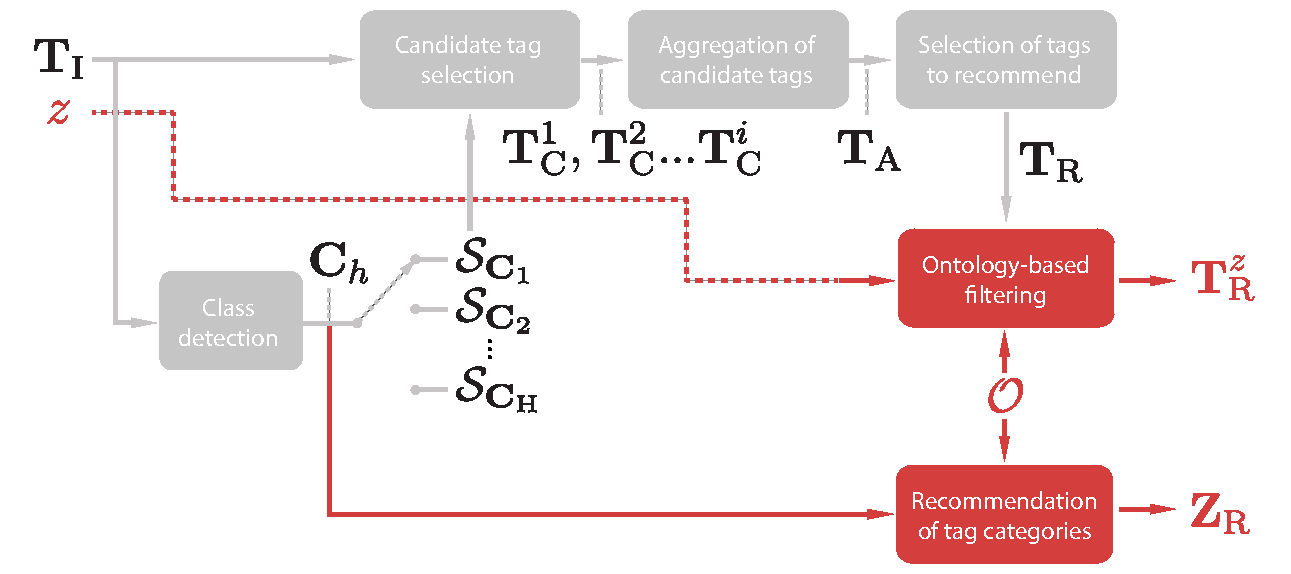
\includegraphics[width=1.0\columnwidth]{ch06_ontology/pics/recommendation_diagram.pdf}
  \caption[Block diagram of the ontology-based tag recommendation system]{Block diagram of the ontology-based tag recommendation system. Note that the ontology-based filtering step takes as input a tag category $\tagCategory$, and outputs a set of recommended tags $\recommendedTagsPerTagCategory$ which depends on $\tagCategory$. Also, further note that for generating $\recommendedTagsPerTagCategory$ and the list of recommended tag categories $\recommendedTagCategories$, the recommendation system relies on the ontology that we described in the previous sections (denoted here as $\ontology$). }
  \label{ontology:fig:diagram}
\end{figure}

\begin{itemize}
\item[i)] The set of recommended tags depends, as usual, on the input tags $\inputTags$ and on the tag-tag similarity matrix $\similarityMatrix_{\audioClass}$ of the audio class $\audioClass$ that is selected after the class detection step. However, in the ontology-based system, the recommendation also takes as input a tag category $\tagCategory$ ($\tagCategory \in \tagCategories$, where $\tagCategories$ is the set of defined tag categories) chosen by the user. %\footnote{To clarify notation in the following sections, we use the lowercase character $\tagCategory$ to refer to a tag category instead of a subscript notation like $\tagCategories_i$.}. 
This tag category is used to filter the output of the class-based system and produce the final set of $\recommendedTagsPerTagCategory$ recommended tags (``Ontology-based filtering'' step in Fig.~\ref{ontology:fig:diagram}).

\item[ii)] Besides outputting a list of recommended tags, the ontology-based tag recommendation system also produces a set of recommended tag categories $\recommendedTagCategories$ that depend on the audio class $\audioClass$ that is detected after the audio class detection step (``Recommendation of tag categories'' step in Fig.~\ref{ontology:fig:diagram}).
\end{itemize} 

%For generating both $\recommendedTagsPerTagCategory$ and $\recommendedTagCategories$, the recommendation system relies on the ontology that we already described (denoted here as $\ontology$). 
%In the following sections we describe more in depth the new steps of the ontology-based tag recommendation system as well as its implementation in terms of user interface.

\subsubsection{Ontology-based filtering of recommended tags}

Given a set of recommended tags $\recommendedTags$ (as produced by the class-based tag recommendation system) and an input tag category $\tagCategory$ chosen by the user, the ontology-based system performs the following operation to generate the final set of recommended tags $\recommendedTagsPerTagCategory$:
\[ \recommendedTagsPerTagCategory = \begin{cases} 
	\postPopulationForTagCategoryL \cup (\recommendedTags \cap \populationForTagCategoryL) & \text{if } |\recommendedTags| > 0 \\
	\postPopulationForTagCategoryL \cup \populationForTagCategoryL &\text{if } |\recommendedTags| = 0 \\
\end{cases}\text{,} \]
where $\populationForTagCategoryL$ is the set of normally-populated tags for the tag category $\tagCategory$, and $\postPopulationForTagCategoryL$ is the set of post-populated tags for $\tagCategory$. 
As it can be observed, if the first steps of the recommendation system (i.e.,~Candidate tag selection, Aggregation of candidate tags and Selection of tags to recommend) are able to generate a set of recommended tags $\recommendedTags$, the system filters that set $\recommendedTags$ by discarding all the tags not populated under the tag category $\tagCategory$. Then, the post-populated tags for the tag category (if any) are added on to the remaining tags in $\recommendedTags$ (duplicates are removed).
On the contrary, if $\recommendedTags$ can not be produced (typically because there are no input tags), the system recommends the union of the post-populated tags (if any) and the normally-populated tags for the corresponding tag category. In this case, normally-populated tags are sorted according to their global frequency of occurrence in the folksonomy of Freesound.

Note that for a given tag category, if there exist post-populated tags in the ontology, these are always recommended in the first place.
Therefore, post-populated tags always take a prominent position in the recommendation. With the exception of the tag category \atag{fso:TypeTag}, only narrow tag categories are post-populated (Sec.~\ref{sec:ontology:population}). The goal of this design choice is that the tags that are post-populated serve more as an example to users that as an actual recommendation. 
For instance, given the tag category \atag{fso:ChordTag}, the tags which are post-populated provide an idea of how to annotate chords (Table~\ref{tab:ontology_tag_categories_most_popular_tags}). Post-population of \atag{fso:ChordTag} includes tags such as \atag{Fmaj7} or \atag{Am9}. These particular chords probably do not suit most of the sounds for which they are recommended, but serve as an example of the syntax that users should follow when introducing chords. Thus, the post-population of tag categories is designed as a way to provide various examples rather than actual recommendations.
This concept also applies, to some extent, to the normally-populated tags that are recommended when $\recommendedTags$ is not generated. In that case, tags serve mostly as an example of what kind of information should be introduced in each tag category.
However, the post-population of the tag category \atag{fso:TypeTag} is performed to promote the usage of a particular set of predefined tags that categorise sounds into rather broad categories (Table~\ref{tab:ontology_tag_categories_most_popular_tags}). By having an extra control over the recommended tags for the \atag{fso:TypeTag} category, we expect that users will annotate the type of their sounds with a more unified vocabulary, using at least one of the tags that we recommend.

Furthermore, note also that the ontology-based tag recommendation system only recommends tags that are populated in the ontology $\ontology$. 
Thus, considering that our ontology is populated with a total of 413 unique tags, the recommendation system only recommends tags from that vocabulary of 413 tags. To overcome that limitation, a more comprehensive population of the ontology should be performed (see the discussion in Sec.~\ref{sec:ontology:conclusion}).


\subsubsection{Recommendation of tag categories}

An extra functionality for the ontology-based tag recommendation system is the suggestion of a set of potentially relevant tag categories $\recommendedTagCategories$ given a set of input tags $\inputTags$. 
This functionality is based on the audio class detection step introduced in the class-based tag recommendation system. 
Given a set of input tags, the classifier is able to predict to which audio class $\audioClass$ a sound belongs to (Sec.~\ref{class:sec:classification_system}).
In the ontology-based tag recommendation system, the predicted audio class $\audioClass$ is directly mapped to the corresponding audio category defined in the ontology (Sec.~\ref{sec:ontology:design}). Then, by considering the range of the object properties in $\ontology$ whose domain matches the predicted audio category, the system is able to generate a list of potentially relevant tag categories $\recommendedTagCategories$ (see below for an example). 

Note that some object properties have as its domain the generic audio class \atag{fso:Sound} (Table~\ref{tab:ontology_tag_categories}). By inheritance, any instance of the audio categories in the lower level of the hierarchy is also an instance of the class \atag{fso:Sound}. Therefore, these object properties are also considered and their corresponding tag categories are recommended. In fact, tag categories whose object property domain is the audio category \atag{fso:Sound} are always recommended.
For example, given a set of input tags whose detected audio category is \atag{fso:Voice}, $\recommendedTagCategories$ will include all tag categories related with \atag{fso:Sound} (e.g.,~\atag{fso:MicrophoneTag}, \atag{fso:TypeTag}, \atag{fso:ProcessingTag}, etc.), as well as all tag categories directly related with \atag{fso:Voice} (\atag{fso:LanguageTag}, \atag{fso:AgeTag} and \atag{fso:GenderTag}).
Those tag categories more related in first place with the detected audio category (i.e.,~not by inheritance), are positioned first in the list of recommended categories. We only make an exception with \atag{fso:TypeTag}, which is always placed in the first position to promote its usage.


\subsubsection{User interface of the annotation system}

The changes introduced in the ontology-based tag recommendation system with respect to the previous class-based system have important implications on the interface for annotating sounds. In Fig.~\ref{ontology:fig:interface}, we show three screenshots of that user interface.
As it can be observed, in an initial stage, the interface provides an input box in which users can start typing tags, and shows the list of all tag categories defined in the ontology (Fig.~\ref{ontology:fig:interface}a).
As soon as users type the first tag in the input box, the tag recommendation system can estimate an audio class $\audioClass$, and provide a recommendation of tag categories $\recommendedTagCategories$. When this happens, the list of tag categories is updated and divided into two parts. The top part lists tag categories in $\recommendedTagCategories$, and bottom part shows the rest of tag categories (Fig.~\ref{ontology:fig:interface}b).

\begin{figure}
  \centering
  \subbottom[]{
    \includegraphics[width=0.87\columnwidth]{ch06_ontology/pics/interface_screenshot_a}}
  \subbottom[]{
    \includegraphics[width=0.87\columnwidth]{ch06_ontology/pics/interface_screenshot_d}}
  \subbottom[]{
    \includegraphics[width=1.0\columnwidth]{ch06_ontology/pics/interface_screenshot_c}}
  \centering
  \caption[Screenshots of the sound annotation interface]{Screenshots of the sound annotation interface using the ontology-based tag recommendation system. 
  Screenshot (a) shows the initial state of the interface, with no input tags introduced. 
  Screenshot (b) shows the interface with a single input tag \texttt{field-recording}.
  Screenshot (c) shows the state of the interface with the input tags $\inputTags=$\{\texttt{music}, \texttt{loop}, \texttt{dubstep}, \texttt{MyBand}\}, and showing tag recommendations for the tag category \texttt{fso:InstrumentTag}. In the latter example, the user has assigned the tags \texttt{music} and \texttt{loop} to the tag category \texttt{fso:TypeTag}, and the tag \texttt{dubstep} to the tag category \texttt{fso:GenreTag}. Notice that the tag \texttt{MyBand} is introduced with no assigned tag category.}
  \label{ontology:fig:interface}
\end{figure}

Users can introduce tags under the tag categories of the ontology by clicking on the tag category names displayed in the interface. When this happens, the tag category name is appended to the input box, and a pop-over appears which includes the recommended tags $\recommendedTagsPerTagCategory$ (Fig.~\ref{ontology:fig:interface}c). 
Similarly to the tag recommendation systems described in previous chapters, recommended tags are sorted according to the scores assigned during the aggregation step of the recommendation process (Sec.~\ref{sec:gen:step_2_aggregation}), but here we only show a maximum of 20 recommended tags.
Users can either choose to add one of the recommended tags or type their own. In either case, the introduced tag is assigned to the selected tag category as an attribute-tag (Sec~\ref{sec:ontology:introduction}).
Note that the vocabulary of tags that can be added under a tag category is not restricted. Hence, users can create new tags and assign them to any tag category.
Note also that multiple tags can be assigned to a single tag category.

Users are not forced to use any of the recommended tag categories, nor forced to use attribute-tags or click on recommended tags. In fact, users are not presented with any recommended tags until they click on one of the tag category names. In this way, the interface guides the annotation process by suggesting information facets and then providing tag recommendations for every information facet on demand, while at the same time it maintains the flexibility of previous tagging systems and allows users to continue tagging in their preferred way (i.e.,~without using attribute-tags).





\section{Evaluation}
\label{sec:ontology:evaluation_method}
% no quantitative definitions of tagging quality, definicio de qualitat de "On Incentive Based Tagging" Xuan S. 2013. the problem is that they refer to broad folksonomies (stability of tags) \cite{Yang2013a}

Here we describe the process we followed to evaluate whether the ontology-based tag recommendation system can better help users to generate comprehensive, coherent, and semantically meaningful resource annotations (when compared to the previous class-based recommendation system of Chapter~\ref{sec:class}).
For that purpose, we designed an online experiment in which participants have to tag a number of sounds from Freesound either using the ontology-based tag recommendation system or the class-based recommendation system. We analyse the logs collected during the experiment and compare both systems by computing a number of metrics.
To complement these results, we also perform a second experiment in which the ontology-based tag recommendation system is deployed in Freesound, and collect logs from real-world usage of the recommendation system. These logs are also analysed, when possible, using the same methodology of the previous experiment.
In the following sections, we describe the experiments and the analysis metrics we use to evaluate our system.

\subsection{Description of online experiments}
\label{sec:ontology:description_of_online_experiments}

\subsubsection{First experiment}

The first experiment was carried out during a time period of 22 days from 7 July 2014 to 13 August 2014. 
The different parts of the experiment are the same as those we used in Chapter~\ref{sec:class} for comparing the class-based tag recommendation system with previous systems (see Sec.~\ref{class:sec:evaluation}). 
Participants were first presented with a page with the instructions of the experiment and corresponding instructions of the tagging interface.
Then, participants had to fill in a questionnaire to collect some basic user data and information about their experience in working with sound libraries, their experience using Freesound and their native language.
After completing the questionnaire, participants could start the sound annotation phase.
We manually selected a pool of 20 sounds from Freesound, equally distributed in the five audio categories introduced in Chapter~\ref{sec:class} (Table~\ref{tab:audio_classes}). 
For each participant in the experiment, we randomly selected 3 sounds per category that had to be tagged. Therefore, participants had to annotate a total of 15 sounds.
The tagging interface was assigned at random per participant. Half of the participants used the ontology-based tag recommendation interface, while the other half used the class-based tag recommendation interface. We will refer to the ontology-based tag recommendation interface as \textsc{Ont}, and to the class-based interface as \textsc{Cla} for short.
In contrast to the experiment described in Chapter~\ref{sec:class}, in this experiment sounds were presented to users along with their original textual descriptions from Freesound. This was added to provide more context to participants and facilitate the tagging task (see discussion in Sec.~\ref{class:sec:user_feedback}).
After annotating the 15 sounds, participants were asked to answer a brief questionnaire to qualitatively evaluate some aspects of the tagging interface. 
We asked to all participants if the tagging interface was easy to understand, and if the tag recommendations were useful. Furthermore, to participants using the \textsc{Ont} interface, we also asked if tag categories were useful, understandable, and if there was enough variety of tag categories. All questions had to be answered using a 5-point scale, ranging from ``strongly disagree'' to ``strongly agree''. Finally, users were given the option to write a comment and provide in this way any other feedback they considered relevant.

Among the 195 participants of the experiment, 109 of them actually completed it.
The percentage of participants that completed the experiment is very similar to that obtained in the online experiment described in Chapter~\ref{sec:class}.
On average, we collected 70 alternative taglines for each sound of the aforementioned pool of 20 sounds, half provided using the \textsc{Ont} interface and half provided using the \textsc{Cla} interface.

\subsubsection{Second experiment}

The second experiment was carried out in Freesound after deploying the on\-to\-lo\-gy-based tag recommendation system as an optional experimental tagging interface. 
During a period of one week from 18 August 2014 to 25 August 2014, Freesound users were given the option to describe their sounds using the ontology-based tagging interface, labelled as an ``experimental tagging interface'' (\textsc{Ont}). Otherwise, users could still use the default tagging interface implemented in Freesound which, at the time of the experiment, was the class-based tagging interface (\textsc{Cla}).
The data collected in this experiment came from the usage of both interfaces in a real-world situation.
Hence, and as opposed to the first experiment, the sounds to be tagged were those uploaded by the users themselves, and we had no control over them.
Because of that, in this experiment, we could not collect multiple taglines per sound. Therefore, some of the analysis metrics that we compute for the first experiment can not be computed for the second experiment. 

During the period of the experiment we collected tagging data for 276 sounds and provided by 91 different Freesound users. 
Almost 70\% of the users chose to use the \textsc{Ont} interface. 
However, not all collected data can actually be included in our analysis.
The reason is that the interface of Freesound allows the description of up to 10 sounds at once, meaning that the information we extract from a single annotation session can correspond to the description of multiple sounds. 
During this process, users may describe sounds in a non-sequential way, and therefore our analysis metrics would not be completely reliable for annotation sessions with multiple sounds. 
For this reason, we only consider the information coming from these annotation sessions in which only one sound was described. As a result, the data that we finally analyse from the second experiment includes tagging data for 135 sounds, provided by 73 different Freesound users. Such data is evenly distributed between the two interfaces (48\% using \textsc{Ont} interface and 52\% using \textsc{Cla} interface).


\subsection{Analysis metrics}
\label{sec:ontology:analysis_metrics}

To analyse the logs collected in the online experiments and compare \textsc{Ont} and \textsc{Cla} tagging interfaces, we define a number of metrics that we divide in three groups. First, we compute simple quantitative metrics to evaluate aspects such as the time participants spend annotating sounds, the length of the tagline  and the number of correctly predicted tags of a given tagline.
Then, we perform a more semantic-oriented analysis in which we look at aspects such as the most commonly used tags and tag categories, and define metrics to roughly quantify the comprehensiveness and coherence of annotations.
Finally, we analyse the qualitative feedback that participants provide through the questionnaire at the end of the first experiment.
%In the following sections we describe and formalise these analysis metrics.


\subsubsection{Quantitative metrics}

We analyse the collected data using some of the quantitative measures already introduced in Chapter~\ref{sec:impact}.
These metrics include the average tagline length ($\metricAverageTaglineLength$), the average tag application time ($\metricAverageTagApplicationTime$), and the average number of correctly predicted tags ($\metricPercentageOfCorrectlyPredictedTags$), formalised in equations~\ref{impact:eq:average_tagline_length} (Sec.~\ref{impact:sec:definition_of_metrics}),~\ref{impact:eq:averae_tag_application_time} (Sec.~\ref{impact:sec:definition_of_metrics}), and~\ref{class:eq:n_accepted_tags} (Sec.~\ref{class:sec:evaluation}), respectively.
In Eq.~\ref{impact:eq:average_tagline_length}, a parameter $n$ is defined to explicitly restrict the set of sounds that are considered for computing the measure on an upload-date basis. In this analysis, we skip this parameter and simply consider a generic set of resources $\resources$. 
Besides these measures, we also include the following two new metrics:

%\item \textit{Average tag application time}: We measure the average time required for assigning a tag to an audio clip, using the average tag application time ($\metricAverageTagApplicationTime$) metric that we defined in Sec.~\ref{impact:sec:methods_cost_of_annotation}, Eq.~\ref{impact:eq:averae_tag_application_time}.
\begin{itemize}
\item \textit{Average time per sound}: Similarly to the average tag application time (Eq.~\ref{impact:eq:averae_tag_application_time}), the average time per sound measures the time required to annotate a sound (i.e.,~to generate a tagline for a sound), averaged over the sounds described in a set of annotation sessions. 
In our analysis, every annotation session corresponds to the description of one sound. Hence, average time per sound can be written as
\begin{equation} \metricAverageTimePerAudioClip =  \frac{1}{|\annotationSessions|}\sum\limits_{\annotationSession \in \annotationSessions}{\durationOfAnnotationSession}, \label{ontology:eq:average_time_per_audio_clip} \end{equation}
where $\durationOfAnnotationSession$ is the duration of an annotation session $\annotationSession$ (in seconds), and $\annotationSessions$ is a set of annotation sessions.

%\item \textit{Average tagline length}: This metric measures the average number of tags assigned to audio clips. A definition for this metric is given in Sec.~\ref{impact:sec:methods_cost_of_annotation}, Eq.~\ref{impact:eq:average_tagline_length}. However, for the current analysis we skip the parameter $n$ of Eq.~\ref{impact:eq:average_tagline_length} and simply consider a generic set of resources $\resources$. Hence, the average tagline length is the average number of tags of $\resources$.
%We already defined this metric in Sec.~\ref{impact:sec:methods_cost_of_annotation}, Eq.~\ref{impact:eq:average_tagline_length}. However, the definition in Eq.~\ref{impact:eq:average_tagline_length} includes the variable $n$ that is used to represent a particular period of time of the analysis. Here, we use a more generic definition such that
%\begin{equation} \metricAverageTaglineLength_\resources =  \frac{1}{|\resources|}\sum\limits_{\resource\in \resources}{|\tagApplicationsPerResourceR|}, \label{impact:eq:average_tagline_length} \end{equation}
%where $\tagApplicationsPerResourceR$ is the set of tag applications involving a resource $\resource$, and $\resources$ is a set of audio clips.

%\item \textit{Average number of correctly predicted tags}: This metric measures the average number of tags from an audio clip that were suggested by the recommendation system during the annotation process of that clip. The average number of correctly predicted tags ($\metricPercentageOfCorrectlyPredictedTags$) is formally defined in Sec.~\ref{impact:sec:methods_cost_of_annotation}, Eq.~\ref{impact:eq:percentage_of_correctly_predicted_tags}. Again, for the current analysis we skip the parameter $n$ of Eq.~\ref{impact:eq:percentage_of_correctly_predicted_tags} and simply consider a generic set of resources $\resources$.

\item \textit{Average percentage of attribute-tags}: We measure the percentage of attri\-bute-tags found in a tagline (i.e.,~the number of tags in a tagline that are introduced with a tag category), and average it over a set of resources. Hence, the average percentage of attribute tags can be formalised as
\begin{equation} \metricPercentageOfAttributeTags = \frac{100}{|\resources|}\sum\limits_{\resource\in \resources}{\frac{| \setOfAttributeTags^{r} |}{ | \tagsOfSoundR | }}, \label{ontology:eq:percentage_of_attribute_tags} \end{equation}
where $\setOfAttributeTags^{r}$ is the set of attribute tags of a resource $\resource$ (i.e.,~tags with category), $\tagsOfSoundR$ is the set of all tags of a resource $\resource$, and $\resources$ is a set of sounds.
This metric can be only computed for data collected from the \textsc{Ont} tagging interface, as attribute-tags are a particular feature of that interface.
\end{itemize}


\subsubsection{Semantic analysis}

The second part of the analysis we perform is focused on semantic aspects of the annotations.
On the one hand, we look at a list of the most common correctly predicted tags for both interfaces (i.e.,~those tags recommended by the system which are most commonly added to the taglines). In this way, we can have an idea of what kind of tags seem to be more useful as recommendations.
On the other hand, we examine which are the most commonly used tag categories in data collected using the \textsc{Ont} interface. From all tags used in every category, we also compute the percentage of them that were actually recommended by the recommendation system (i.e.,~correctly predicted). In this way, we can have an idea of which are the most useful tag categories and about how effective the recommendation system is in every category.
Also, in order to have an indication of whether the tag categories included in the ontology were enough for annotating the sounds, we have a look at those tags that were introduced without category (non-attribute-tags), and see if these could have been categorised under the existing categories or some of them might require the inclusion of new ones.
The latter analyses are also only applicable to the \textsc{Ont} tagging interface.

Besides looking at the previous aspects, we further define two analysis metrics which provide an estimation of the comprehensiveness and coherence of sound annotations generated with both interfaces. These two metrics are based on the analysis of the alternative taglines that we collected for every sound in the first experiment: %Hence, these can not be applied to the data collected from the second experiment. What follows is the definition of these metrics.

\begin{itemize}
\item \textit{Annotation comprehensiveness}: %The purpose of annotation comprehensiveness is to give an orientative measure of how comprehensive a tagline for a particular resource is. 
Comprehensiveness is measured in terms of the number of distinct information facets that are covered in a tagline. In essence, the more information facets are annotated, the more comprehensive the tagline is considered to be.
For each sound annotated in the first experiment, we collected an average of 70 alternative taglines, approximately half of them generated with the \textsc{Ont} interface and half with the \textsc{Cla} interface (Sec.~\ref{sec:ontology:description_of_online_experiments}).
Considering all the alternative taglines for a given sound, we build an annotation ground truth for that sound, which is then used to evaluate how comprehensive individual taglines are. 

To construct the ground truth for a given sound, we aggregate the individual tags of all alternative taglines into a single set of tags, and manually group them into several information facets. The category of attribute-tags is removed, so that we only add the actual tag to that list. Then, to group the list of tags, we follow a similar process to that described for the definition and population of the tag categories in the ontology (Sec.~\ref{sec:ontology:population}). Given that, in this case, the grouping of tags is performed with the actual sound as a reference, tags can be grouped according to the kind of information they describe in the context of that particular sound. Hence, the process becomes simpler and less ambiguous.
As a result, we obtain a number of information facets with a set of tags classified into them. 
Given the ground truth and a tagline for a sound, the comprehensiveness of a tagline is computed by comparing the number of information facets covered by the tagline (i.e.,~the number of facets from the ground truth for which there is at least one tag in the tagline), with the total number of possible information facets defined in the ground truth.
Hence, given the intermediate function
\[ covered(\mathbf{X},\mathbf{Y}) = \begin{cases} 
	1 & \text{if } |\mathbf{X} \cap \mathbf{Y}| > 0 \\
	0 & \text{if } |\mathbf{X} \cap \mathbf{Y}| = 0 \\
\end{cases}\text{,}\]
annotation comprehensiveness is defined as
\begin{equation} \metricAnnotationComprehensiveness = \frac{1}{|\groundTruthForResourceR|}\sum\limits_{\tags_\text{IF} \in \groundTruthForResourceR}{covered(\tagsOfSoundR, \tags_\text{IF})}
\text{,} 
\label{ontology:eq:annotation_comprehensiveness} \end{equation}
where $\tagsOfSoundR$ is the tagline of a resource $\resource$, $\groundTruthForResourceR$ is the ground truth of a resource $\resource$, and $\tags_\text{IF}$ is a set of tags corresponding to one of the information facets defined in $\groundTruthForResourceR$.
Using this measure, we can estimate how comprehensive are, individually, each of the alternative taglines provided for every annotated sound. Then, we can compare the annotation comprehensiveness of \textsc{Ont} and \textsc{Cla} interfaces by averaging this measure over all the taglines generated with each interface.

\item \textit{(In)coherence in annotations}: To evaluate the coherence of a set of alternative taglines for a given sound we, in fact, define a measure of incoherence.
Incoherence is measured in terms of the variety of tags that are used to convey a unique semantic meaning (or audio property).
The more variety of tags is used to describe a particular property in a set of taglines for a given sound, the more incoherent these taglines are considered to be. 
For example, given an audio recording of a musical instrument playing a chord, a set of taglines that feature tags like \atag{DMaj}, \atag{D-major}, \atag{Dmajor} and \atag{DM} to indicate the chord, is more incoherent than another set of taglines in which the chord is always indicated with either \atag{DMaj} or \atag{Dmajor} (using fewer variations). In a sense, the incoherence in annotations reflects the agreement on how to annotate particular audio properties among the participants that generated the taglines.
Similarly to annotation comprehensiveness, we estimate the incoherence in annotations by building an annotation ground truth for each of the sounds annotated in the first experiment. Then, this ground truth is used to estimate the incoherence of the taglines of the corresponding sound.
Hence, incoherence in annotations can only be computed on data collected in the first experiment.

The annotation ground truth that we build for this measure is different to that built for annotation comprehensiveness.
Here, given a sound, we also aggregate the individual tags of all alternative taglines into a single set of tags, but instead of grouping them into rather broad information facets, we group together those tags that convey the same or very similar information.
For example, we group together tags like \{\atag{Funk}, \atag{funk}, \atag{funky}\}, which denote the same music genre, tags like \{\atag{distortion}, \atag{smooth-distortion}, \atag{distorted},\atag{overdrive}\}, which all describe a very similar audio processing effect, or tags like \{\atag{talking}, \atag{speak}, \atag{talk}, \atag{chatting}, \atag{speaking}\}, which refer to the same activity. Tags with no other equivalent (or very similar) tags are not considered in the ground truth.
As a result, the annotation ground truth for a sound consists of a list of sets of tags that are almost equivalent from a semantic point of view (i.e.,~a list of \emph{synsets}\footnote{To simplify explanations, we adopt the terminology used in WordNet~\citep{Miller1995}, which refers to a set of synonyms as a ``synset''. In our case, we use the term synset with a slightly broader meaning, as tags are not strictly grouped because of being synonyms, but because of featuring high semantic equivalence.}). 
Considering the ground truth for a sound and a set of alternative taglines, we iterate over its identified synsets and count how many of the tags in the synset are present in the set of taglines. Averaging that value over the different synsets, we obtain an indication of the incoherence in a set of taglines. %Note that the measure we compute is, in fact, a measure of ``incoherence'' in annotations, as the higher the result, the less coherent the taglines are considered to be. Nevertheless, 
The measure can be formalised as 
\begin{equation} \metricCoherenceInAnnotations = \frac{1}{|\groundTruthForResourceR|}\sum\limits_{\tags_\text{SY} \in \groundTruthForResourceR}{|\tagsOfSoundR_\text{TL} \cap \tags_\text{SY}| }
\text{,} 
\label{ontology:eq:choerence_in_annotations} \end{equation}
where $\tagsOfSoundR_\text{TL}$ is the union of all tags from a set of taglines of a resource $\resource$, $\groundTruthForResourceR$ is the annotation ground truth of a resource $\resource$, and $\tags_\text{SY}$ is a set of tags corresponding to one of the synsets defined in $\groundTruthForResourceR$.
Using this measure, we can estimate how incoherent a set of taglines is for a given sound. By computing this measure over sets of taglines collected with the \textsc{Ont} and \textsc{Cla} interfaces, we can compare them in terms of incoherence in resulting annotations.

\end{itemize}

\subsubsection{Qualitative feedback}
To analyse the qualitative feeback provided by users we compute the average over the responses of the different questions answered in the 5-point scale (see Sec.~\ref{sec:ontology:results_qualitative_feedback}), and relate these with the results of the quantitative and semantic analysis. 
Furthermore, we compare the responses of these questions which are common to participants using both interfaces.
Finally, we comment on the extra qualitative feeback that we collected in the form of textual comments.


\subsection{Analysis methodology}
\label{sec:ontology:analysis_methodology}

The analysis we perform is mainly centred on the data collected from the first experiment. This is because, as we have seen, the nature of the second experiment does not allow us to compute all the metrics listed above. Hence, the analysis of the data from the second experiment is used, whenever available, as a complement to the analysis of the first experiment. Nevertheless, with the exception of some metrics, we use the same methodology to analyse the data collected from both experiments. In general, we consider data generated with the \textsc{Ont} interface separated from data generated with the \textsc{Cla} interface, and then compare the results of the different metrics. Statistical significance is assessed using the Mann-Whitney U test with a significance level of 0.05~\citep{Corder2009}.
%test was previously cited as ~\citep{Mann1947}.

Before computing the analysis measures described above, we filter the collected data to remove potentially irrelevant or noisy logs.
The filter is applied at the sound level, meaning that we discard the information from individual sounds that do not pass the filter.
The first filter we compute operates on the duration of annotation sessions for sounds.
We discard annotation sessions based on the interquartile range of their duration.
Let $q_1$ be the first quartile and $q_3$ be the third quartile of the durations of annotation sessions, we discard sounds whose annotation session duration is outside the range $[q_1 - 3(q_3 - q_1), q_3 + 3(q_3 - q_1)]$. In practice, this means that we only consider data corresponding to sounds that were annotated in less than 260 seconds.
We apply a second filter in which we discard all sound annotation sessions in which there are no logged \emph{calls} to the tag recommendation system. In these sessions, no tag recommendations were provided to the user. This might happen because of different reasons (see below).
%We consider that annotation sessions that do not comply with both filters are not reliable for our analysis. 
%In some cases, we also report results that consider annotation sessions without applying that filter. We do that when it is useful to illustrate some particular aspects of our analysis.


After applying the filter to all collected annotation sessions of the first experiment, we see that 69\% pass the filter. 
Most of the annotation sessions comply with the timing restriction (97\%), but only 72\% feature at least one call to the recommendation system. 
Annotation sessions that do not pass the filter mostly correspond to sessions using the \textsc{Ont} interface.
%This is because only 42\% of sessions using the \textsc{Ont} interface feature at least one call to the recommendation system.%, whereas virtually all \textsc{Cla} sessions interface (99\%) feature at least one call.
This observation can be partially explained because, when using the \textsc{Ont} interface, tags are only recommended when users click on the tag categories (Sec.~\ref{sec:ontology:tag_recommendation}).
Conversely, when using the \textsc{Cla} interface, tags are automatically recommended when users start typing.
As a consequence, it can happen, particularly when using the \textsc{Ont} interface, that no tags are recommended at all.
We observe that only 42\% of annotation sessions using the \textsc{Ont} interface feature at least one call to the recommendation system.
Possible reasons for that could be that users do not properly understand how the interface works or that they do not think that tag categories are meaningful or necessary.
%This could be either because users do not properly understand how the interface works, because they do not think that tag categories are useful, or even because of technical problems causing errors in the interface.
Overall, the fact that less than half of the annotation sessions using the \textsc{Ont} interface pass both filters indicates that a lot of participants, for whatever reason, did not take advantage of the features of the interface as we expected. 
When applying the filter to the data from the second experiment, we observe practically the same percentages.
Therefore, one interesting aspect of the \textsc{Ont} interface that should be further investigated is why such a big percentage of users does not take advantage of recommendation functionalities as we expected (see discussion in Sec.~\ref{sec:ontology:conclusion}).


\section{Results}
\label{sec:ontology:results}

\subsection{Quantitative metrics}
\subsubsection{Average time per sound}

%EXP 1
%Statistical test (alpha=0.050000):
%	cur: avg:60.9222 std:41.3242 med:51.5000 - 784 values
%	ont: avg:108.5625 std:55.8287 med:95.0000 - 272 values
%	delta: 47.640306 test: 47992.000000 p_value 5.279e-42

%EXP 2
%Statistical test (alpha=0.050000):
%	cur: avg:155.6167 std:125.0467 med:121.0000 - 60 values
%	ont: avg:301.0625 std:188.6306 med:254.5000 - 32 values
%	delta: 145.445833 test: 500.000000 p_value 8.259e-05

The average time per sound $\metricAverageTimePerAudioClip$ reveals that sound annotations tend to require more time when using the \textsc{Ont} interface.
In particular, we observe a statistically significant average increase of 48 seconds ($\pvalue = 5.28\cdot 10^{-42}$). Fig.~\ref{fig:ontology:time_per_sound} shows the probability density function of the time per sound for both interfaces. The average time per sound is of 60 seconds for participants using the \textsc{Cla} interface, and of 109 seconds for participants using the \textsc{Ont} interface.
Similarly, when looking at real-world data from the second experiment, we also observe that users that choose the \textsc{Ont} interface spend more time annotating their sounds. In this case, the average time per sound of both interfaces is significantly higher than in the first experiment (156 seconds for \textsc{Cla} and 301 seconds for \textsc{Ont}), and so it is the difference between them (145 seconds, $\pvalue = 8.27\cdot 10^{-5}$).
This can be explained because, in the second experiment, users do not only have to annotate sounds, but also have to provide other information which is required by the Freesound uploading interface. This information includes a name for the sound, a textual description, a license and, optionally, geolocation and pack\footnote{In Freesound, sounds can be explicitly grouped in packs that users define.} information.
Furthermore, the increased difference between both interfaces observed in the second experiment can also be due to users experimenting with the interface to understand how it works. In the first experiment, before starting to annotate sounds, users were provided with instructions for the corresponding interface. Conversely, in Freesound, these instructions were not provided beforehand, and could only be accessed through a link that was provided during the annotation process.

\begin{figure}[t]
  \centering
  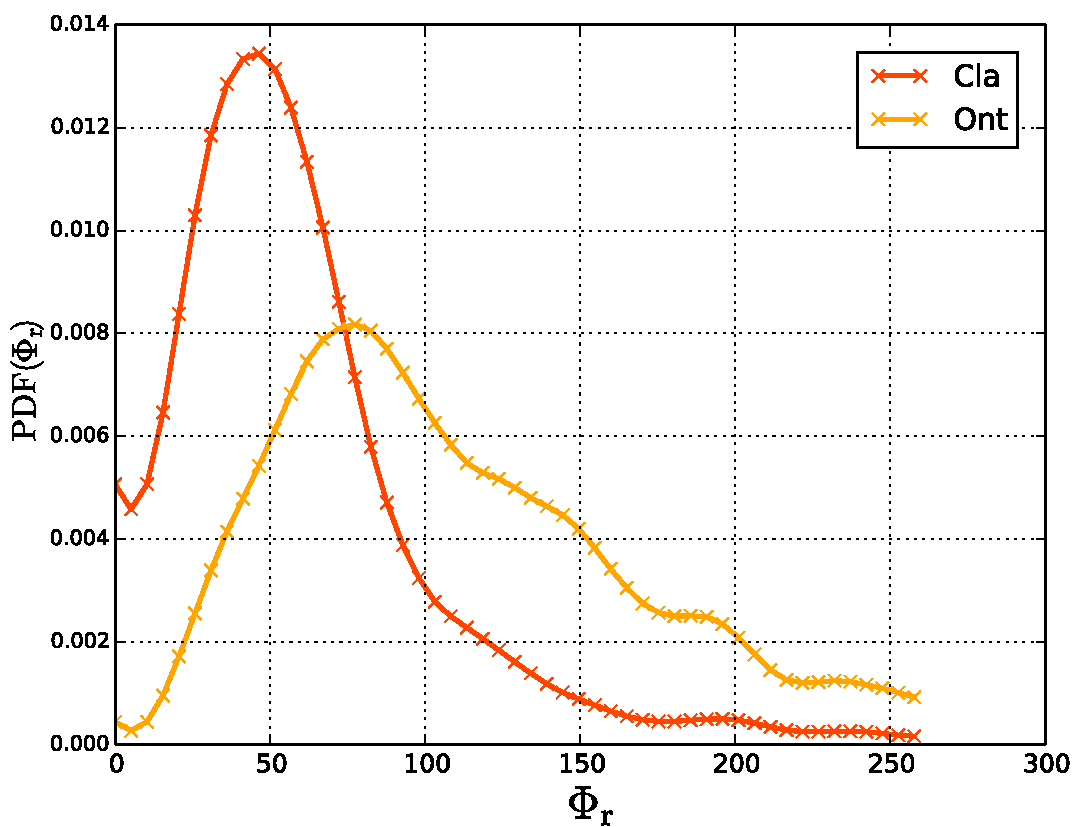
\includegraphics[width=\figSizeMidLarge]{ch06_ontology/pics/time_per_sound_pdf}
  \caption[Probability density function of the time per sound]{Probability density function of the time per sound $\metricAverageTimePerAudioClip$ with \textsc{Ont} and \textsc{Cla} interfaces. Curves are smoothed using a Hann window of 11 points.}
  \label{fig:ontology:time_per_sound}
\end{figure}

\subsubsection{Average tag application time}

% EXP 1
%Statistical test (alpha=0.050000):
%	cur: avg:11.0031 std:9.1202 med:8.7500 - 784 values
%	ont: avg:20.4508 std:17.4559 med:18.0000 - 272 values
%	delta: 9.447769 test: 48526.500000 p_value 2.82e-41

% EXP 2
%Statistical test (alpha=0.050000):
%	cur: avg:19.3058 std:23.4081 med:11.0682 - 60 values
%	ont: avg:47.0138 std:46.4678 med:33.3246 - 32 values
%	delta: 27.708056 test: 387.000000 p_value 1.344e-06

The average tag application time $\metricAverageTagApplicationTime$ features a very similar behaviour to that observed with $\metricAverageTimePerAudioClip$.
Participants of the first experiment need, on average, 11 seconds for assigning a tag using the \textsc{Cla} interface, and 20 seconds using the \textsc{Ont} interface. The increase of 9 seconds is statistically significant ($\pvalue = 2.82\cdot 10^{-41}$).
Similarly, in the second experiment, both the increase of the average tag application time is higher (28 seconds, $\pvalue = 1.34\cdot 10^{-6}$), and also the average times for both interfaces (19 seconds for \textsc{Cla} and 47 seconds for \textsc{Ont}).
Besides being in line with the previous measure, these results suggest that the extra time that users require for annotating sounds with the \textsc{Ont} interface is not because the generated taglines are longer, but because the assignment of each tag requires more time. 
%However, this aspect is better represented in the following metric.


\subsubsection{Average tagline length}

% EXP 1
%Statistical test (alpha=0.050000):
%	cur: avg:6.2398 std:2.9034 med:6.0000 - 784 values
%	ont: avg:6.6140 std:3.7790 med:6.0000 - 272 values
%	delta: 0.374175 test: 105296.500000 p_value 0.3789

% EXP 2
%Statistical test (alpha=0.050000):
%	cur: avg:12.0667 std:6.5799 med:11.0000 - 60 values
%	ont: avg:9.0938 std:5.7682 med:8.5000 - 32 values
%	delta: -2.972917 test: 720.000000 p_value 0.02447

The observations on the average tagline length that we can make by analysing the data from the first experiment confirm the previous suggestion that taglines do not tend to be longer for participants using the \textsc{Ont} interface. Although the average tagline length is slightly higher (6.61 tags for \textsc{Ont} interface and 6.24 tags for \textsc{Cla} interface), the difference is not statistically significant.
However, the results of the average tagline length computed for the second experiment are surprising. In this case, we observe that taglines using the \textsc{Cla} interface are in fact longer that those generated with the \textsc{Ont} interface (12.07 tags and 9.10 tags respectively, $\pvalue = 2.45\cdot 10^{-2}$).
The reason for this behaviour is not clear. One possible explanation is that with the usage of attribute-tags, sound annotations may appear to be more specific and complete while using fewer tags. Hence, users might feel that the description is good enough using fewer tags. In practice, the \textsc{Ont} interface merges tag categories and actual tags in the same space (see Fig.~\ref{ontology:fig:interface}), and this might cause the perception that the tagline is longer than it actually is.
%Another possible explanation could be the inexperience of users with the \textsc{Ont} interface.



\subsubsection{Average number of correctly predicted tags}

% EXP 1
%Statistical test (alpha=0.050000):
%	cur: avg:2.4834 std:2.1618 med:2.0000 - 784 values
%	ont: avg:2.5956 std:2.0629 med:2.0000 - 272 values
%	delta: 0.112170 test: 101629.500000 p_value 0.1215

% EXP 2
%Statistical test (alpha=0.050000):
%	cur: avg:3.3000 std:2.9569 med:3.0000 - 60 values
%	ont: avg:2.9688 std:2.4935 med:2.0000 - 32 values
%	delta: -0.331250 test: 915.000000 p_value 0.3563


The analysis of the average number of correctly predicted tags does not reveal a significant difference when comparing interfaces.
Sounds annotated with the \textsc{Cla} interface feature an average of 2.48 correctly predicted tags, which is very similar to that obtained in our previous evaluation of the \textsc{Cla} recommendation method (Chapter~\ref{sec:class}, Table \ref{tab:results_general_ub}), and of the impact of the tag recommendation system (Chapter~\ref{sec:impact}, Sec.~\ref{impact:sec:percentage_correcly_predicted_tags_results}).
Sounds annotated with the \textsc{Ont} interface feature a slightly higher average of 2.60 correctly predicted tags, but the difference is not statistically significant ($\pvalue = 1.22\cdot 10^{-1}$).
On the data collected for the second experiment, we again observe similar results with no statistically significant differences between interfaces (average of 3.30 and 2.97 correctly predicted tags for \textsc{Ont} and \textsc{Cla} interfaces, respectively, $\pvalue = 3.56\cdot 10^{-1}$).
What these results suggest is that the grouping of tags into tag categories and the recommendation of post-populated tags provided by the \textsc{Ont} interface does substantially not impact the number of tags from taglines that are correctly predicted by the recommendation system. 

Similarly to what we did in Chapter~\ref{sec:class}, we analysed if there is a correlation between the average number of correctly predicted tags and users' expertise and language (Sec.~\ref{class:sec:accepted_tags_results}). In particular, we consider the results from the first experiment and divide collected logs between groups of experienced and non-experienced participants, and native and non-native English speakers. Accordingly to what we describe in Sec.~\ref{class:sec:accepted_tags_results}, we observe here small increases in the number of correctly predicted tags for both expert and native speaker participants (in both interfaces). However, as opposed to the previous analyses, the differences in this case do not appear to be statistically significant.
Further research should be carried out in order to make stronger claims regarding that matter.
%Therefore, this result partially questions our previous specific findings regarding that matter and should be further researched. 


\subsubsection{Average percentage of attribute-tags}

% EXP 1
%Basic stats:
%	Percentage of tags with category: avg:0.7244 std:0.3521 med:1.0000 - 272 values
%41.30\% of sounds have at least one semantic tag (no filtering)

%Correlation with user experience
%Labels index:
%	1: Non experienced,ont
%	2: Experienced,ont
%General stats:
%	Non experienced,ont      0.6247 (0.4244) - 63 values
%	Experienced,ont          0.7545 (0.3212) - 209 values
%Statistical test data:
%-           1           2           
%1           -           3.855e-02   
%2           3.855e-02   -           

% EXP 2
% Basic stats:
%	Percentage of tags with category: avg:0.6359 std:0.3988 med:1.0000 - 32 values
%57.14\% of sounds have at least one semantic tag (no filtering)

Considering the taglines generated with the \textsc{Ont} interface for our first experiment, we observe that an average of 72\% of the tags are introduced under a tag category (i.e.,~are attribute-tags). In the second experiment, this percentage is slightly lower, at 65\%.
This means that a significant number of tags from taglines are contextualised in one of the defined tag categories of the ontology, and therefore their semantic value is effectively improved.
However, it is important to note that these percentages are achieved when considering filtered data as described in Sec.~\ref{sec:ontology:analysis_methodology}. This filter removes, among others, data from annotation sessions in which participants do not take advantage of the tagging interface as we expected. %Hence, the average percentage of attribute-tags is greatly affected by the filter. 
In Fig.~\ref{fig:ontology:percentage_of_attribute_tags}, we show the histogram of the number of attribute tags per tagline when considering unfiltered data for the first experiment. What we observe now is that more than half of the taglines (59\%) feature no attribute-tags, whereas other taglines tend to have between 1 and 7 attribute-tags. A similar observation can be made in the second experiment, with 43\% of taglines featuring no attribute-tags.
These results suggest that the tagging interface should better encourage the usage of attribute-tags.

\begin{figure}[t]
  \centering
  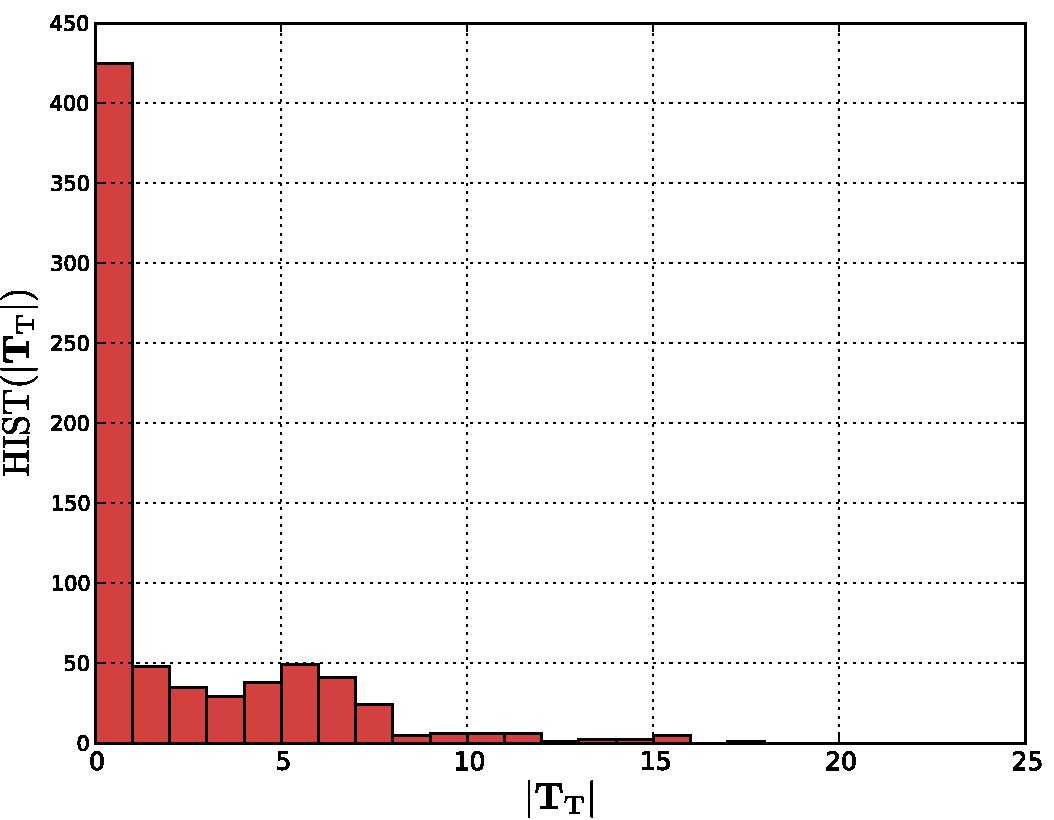
\includegraphics[width=\figSizeMidLarge]{ch06_ontology/pics/number_of_semantic_tags_histogram_no_filter}
  \caption[Histogram of the number of attribute-tags per tagline]{Histogram of the number of attribute-tags per tagline $|\setOfAttributeTags|$ in the first experiment (including unfiltered data).}
  \label{fig:ontology:percentage_of_attribute_tags}
\end{figure}

To complement these results, we analyse if there is a correlation between users' expertise and the percentage of attribute-tags. We observe that experienced users tend to include, on average, 13\% more attribute-tags than non-experienced users, that difference being statistically significant ($\pvalue = 3.86\cdot 10^{-2}$). This might be explained because experienced users better understand the advantages that attribute-tags provide in terms of description accurateness and further retrieval possibilities.


\subsection{Semantic analysis}

\subsubsection{Most common correctly predicted tags}

\begin{table}
\ra{1.2}
\begin{center}
\footnotesize
\begin{tabular}{@{}p{2cm}p{5cm}p{5cm}@{}}
\toprule
\textbf{Experiment} & \textsc{Ont} \textbf{interface} & \textsc{Cla} \textbf{interface} \\
\midrule
First & field-recording, voice, synth, condenser, single-note, fx, loop, soundscape, stereo, ambiance, 120bpm, electronic, percussive-hit, city, mezzo-forte, fast-attack, processed, mono, male, rhythm & field-recording, electronic, loop, synth, voice, people, rain, male, bell, child, weather, female, ring, nature, bells, vocal, beat, ambience, writing, city \\
%First & field-recording~(32), voice~(31), synth~(26), condenser~(23), single-note~(23), fx~(23), loop~(20), soundscape~(17), stereo~(17), ambiance~(15), 120bpm~(13), electronic~(12), percussive-hit~(11), city~(11), mezzo-forte~(11), fast-attack~(10), processed~(10), mono~(9), male~(9), rhythm~(8) & field-recording~(57), electronic~(46), loop~(39), synth~(35), voice~(32), people~(25), rain~(23), male~(22), bell~(22), child~(22), weather~(22), female~(21), ring~(21), nature~(21), bells~(21), vocal~(20), beat~(20), ambience~(19), writing~(19), city~(19) \\
Second & fx, soundscape, field-recording, talking, horror, condenser, stereo, male, english, voice, loop, summer, atmosphere, neumann, crowd, pop, distortion, suspense, female, violin & drums, drum, atmosphere, fx, ten, dance, house, ambiance, gloomy, deep, down, cavern, ambient, rave, chime, airplane, electronic, monster, sub, 0 \\
%Second & fx~(3), soundscape~(3), field-recording~(3), talking~(2), horror~(2), condenser~(2), stereo~(2), male~(2), english~(2), voice~(2), loop~(2), summer~(1), atmosphere~(1), neumann~(1), crowd~(1), pop~(1), distortion~(1), suspense~(1), female~(1), violin~(1) & drums~(2), drum~(2), atmosphere~(1), fx~(1), ten~(1), dance~(1), house~(1), ambiance~(1), gloomy~(1), deep~(1), down~(1), cavern~(1), ambient~(1), rave~(1), chime~(1), airplane~(1), electronic~(1), monster~(1), sub~(1), 0~(1) \\
\bottomrule
\end{tabular}
\caption[Most common correctly predicted tags]{First 20 most common correctly predicted tags for the first and second experiments and for \textsc{Ont} and \textsc{Cla} interfaces. 
%In parenthesis we indicate the total number of tag occurrences.
}
\label{tab:ontology_most_correctly_predicted_tags}
\end{center}
\end{table}

The most common correctly predicted tags for both experiments and interfaces are listed in Table~\ref{tab:ontology_most_correctly_predicted_tags}.
Looking at the tags of the first experiment, we observe that, regardless of the interface, an important number of tags have a semantic meaning that would belong to the \atag{fso:TypeTag} category (e.g.,~\atag{field-recording}, \atag{voice}, \atag{ambiance}). Other common tags belong to well defined musical concepts (e.g.,~\atag{loop}, \atag{synth}, \atag{electronic}, particularly in the \textsc{Ont} interface). Overall, both interfaces present similar (or very related) most common correctly predicted tags. In fact, 20\% of the first 50 most common correctly predicted tags in \textsc{Ont} and \text{Cla} interfaces are \emph{exactly} the same. 
This can be explained because the pool of sounds to annotate in the first experiment was limited to 20 sounds, and the concepts to annotate are determined by the sounds. 
However, of particular interest is the case of very specific tags such as \atag{120bpm}, \atag{mezzo-forte} and \atag{fast-attack}, which are included in the list of most common correctly predicted tags for the \textsc{Ont} interface. 
These tags are post-populated under the \atag{fso:TempoTag}, \atag{fso:DynamicsTag} and \atag{fso:EnvelopeTag} categories respectively (Table~\ref{sec:ontology:population}), and are therefore always recommended when using the \textsc{Ont} interface. If these tags were not recommended, users would presumably employ different variations of the same tags (e.g.,~\atag{mezzoforte} instead of \atag{mezzo-forte}) that would prevent them from being amongst the most common correctly predicted tags unless these were very obvious. In fact, we hypothesise that this is what happens for the tags that belong to the \atag{fso:TypeTag} category which, as we commended before, are an important part of the most common correctly predicted tags in both interfaces. We can see, for example, that the tag \atag{voice} takes the second position in the \textsc{Ont} interface, and that the other tags in the list have completely different meanings. Interestingly, in the \textsc{Cla} interface, we see how two tags that present a notable semantic overlap (\atag{voice} and \atag{vocal}), are both in the list of most common correctly predicted tags (in the fifth and sixteenth position).

If we look at the most common correctly predicted tags of the second experiment, we observe some differences.
Here, we do not observe such similarity between tags from both interfaces (only 8\% are common amongst the first 50 most common correctly predicted tags).
This was to be expected, as the sounds described in this experiment are not controlled, hence the potentially relevant concepts to annotate are not necessarily comparable between interfaces.
However, in the tags from the \textsc{Ont} interface, we still observe a great presence of post-populated tags from the \atag{fso:TypeTag} category, which is not observed in the \textsc{Cla} interface (e.g.,~\atag{voice}, \atag{soundscape}, \atag{field-recording}).
Overall, these results suggest that \atag{fso:TypeTags} tags are more useful as tag recommendations in the \textsc{Ont} interface, and that post-population in general seems to contribute in the coherence of the vocabulary.



\subsubsection{Usage of tag categories}

In this section we have a look at the most commonly used tag categories in both experiments, and at the percentage of the tags introduced in every category that were correctly predicted by the recommendation system (Table~\ref{tab:tag_categories_usage}).
Usage is computed as the percentage over the total number of taglines (of the \textsc{Ont} interface) that feature at least one attribute-tag of a particular tag category.
We observe that the most used tag categories are, in general, those which are applicable to virtually any kind of sound (first rows of Table~\ref{tab:tag_categories_usage}).
The tag categories that are highly used depend on the kinds of sounds being annotated (e.g.,~music sounds require music-related tag categories). Therefore, the comparison between tag categories usage for both experiments is not a priori very meaningful. However, we observe that there is a significant correlation between the ranking of tag categories usage in both experiments (second and third columns of Table~\ref{tab:tag_categories_usage}).
To asses this correlation, we employ the Spearman's rank correlation coefficient~\citep{Corder2009} and observe a correlation coefficient of $\spearmanCorrelationCoefficient=0.745$ with a $\pvalue$-value of $\pvalue = 1.24\cdot 10^{-5}$. We hypothesise that this correlation can be explained by the presence of generic tag categories that can be relevant to different kinds of sounds.
Overall, it is interesting that in both experiments, the \atag{fso:TypeTag} is the most used tag category. As we explained before, our design puts a special emphasis on the \atag{fso:TypeTag} category (Sec.~\ref{sec:ontology:population}). 
Hence, the broad presence of this category in sound descriptions is one successful outcome of using the \textsc{Ont} interface.
% the rank correlation coefficient was previously cited as hogg1995

Another aspect that we examine is the percentage of correctly predicted tags introduced under every tag category. To evaluate this, for every tagline we take into account all introduced tags from each tag category and compute the percentage of these that were recommended by the system during the annotation session. This value is then averaged over all taglines (fourth and fifth columns of Table~\ref{tab:tag_categories_usage}). A high percentage indicates that many of the tags used under a category come from system recommendations. %, while a low percentage indicates that tags introduced under that category are not taken from tag recommendations.
Again, we observe that there is a high correlation between the percentage of correctly predicted tags per category in both experiments ($\spearmanCorrelationCoefficient=0.906$, $\pvalue = 2.19\cdot 10^{-7}$), meaning that tag categories feature similar percentages in both experiments.
Particularly relevant are those categories in which both the percentage of usage and the percentage of correctly predicted tags are high (Table~\ref{tab:tag_categories_usage}). In these cases, it can be hypothesized that the \textsc{Ont} interface successfully contributes in the homogenisation of the information facet of the particular tag category, as users reuse tags suggested by the recommendation system rather than creating new ones.
This is the case of the tag categories in the first rows of Table~\ref{tab:tag_categories_usage}, and particularly of the \atag{fso:TypeTag} category, which shows a wide usage and wide reuse of the tags recommended by the system.

\begin{table}
\ra{1.2}
\begin{center}
\footnotesize
\begin{tabular}{@{}lcccc@{}}
\toprule
 & \multicolumn{2}{c}{\textbf{\% usage}} & \multicolumn{2}{c}{\textbf{\% correctly predicted}} \\
\textbf{Tag category} & \textbf{First exp.} & \textbf{Second exp.} & \textbf{First exp} & \textbf{Second exp.} \\
\midrule
\texttt{fso:TypeTag} & 61.40 & 50.00 & 93.36 & 100.00 \\
\texttt{fso:InstrumentTag} & 36.76 & 21.88 & 58.63 & 80.00 \\
\texttt{fso:WhatTag} & 22.79 & 28.12 & 53.67 & 69.44 \\
\texttt{fso:MicrophoneTag} & 20.96 & 28.12 & 40.35 & 66.67 \\
\texttt{fso:RecordingTag} & 18.01 & 40.62 & 85.14 & 85.71 \\
\texttt{fso:ProcessingTag} & 18.01 & 12.50 & 65.40 & 100.00 \\
\texttt{fso:MoodTag} & 14.71 & 18.75 & 42.86 & 40.00 \\
\texttt{fso:GearTag} & 13.97 & 18.75 & 17.54 & 33.33 \\
\texttt{fso:ActionTag} & 13.60 & 25.00 & 51.35 & 85.71 \\
\texttt{fso:WhereTag} & 12.87 & 21.88 & 50.65 & 44.44 \\
\texttt{fso:GenderTag} & 11.40 & 18.75 & 90.38 & 100.00 \\
\texttt{fso:NoteTag} & 11.03 & 0.00 & 28.33 & - \\
\texttt{fso:TempoTag} & 10.66 & 3.12 & 44.83 & - \\
\texttt{fso:SoftwareTag} & 9.56 & 21.88 & 1.96 & 25.00 \\
\texttt{fso:OnomatopeiaTag} & 9.19 & 0.00 & 41.67 & - \\
\texttt{fso:MaterialTag} & 8.82 & 9.38 & 77.50 & 100.00 \\
\texttt{fso:DynamicsTag} & 7.72 & 0.00 & 100.00 & - \\
\texttt{fso:EnvelopeTag} & 7.72 & 3.12 & 100.00 & 100.00 \\
\texttt{fso:AgeTag} & 6.99 & 6.25 & 66.67 & - \\
\texttt{fso:LanguageTag} & 6.62 & 15.62 & 50.00 & 75.00 \\
\texttt{fso:KeyTag} & 5.51 & 0.00 & 13.33 & - \\
\texttt{fso:GenreTag} & 4.78 & 9.38 & 33.33 & 50.00 \\
\texttt{fso:ArticulationTag} & 4.41 & 0.00 & 83.33 & - \\
\texttt{fso:WhenTag} & 3.31 & 12.50 & 41.67 & 50.00 \\
\texttt{fso:MeterTag} & 2.94 & 3.12 & 100.00 & 100.00 \\
\texttt{fso:ChordTag} & 2.57 & 0.00 & 42.86 & - \\
\bottomrule
\end{tabular}
\caption[Percentage of usage and percentage of correctly predicted tags per tag category]{Percentage of usage of the different tag categories in the first and second experiments, and percentage of correctly predicted tags for every category and experiment. Tag categories are sorted according to their percentage of usage in the first experiment. Note that this table only includes data gathered with the \textsc{Ont} interface, as the concept of tag categories is not present in the \textsc{Cla} interface.}
\label{tab:tag_categories_usage}
\end{center}
\end{table}

\subsubsection{Most commonly used tags without tag category}

In Table~\ref{tab:ontology_most_common_non_attribute_tags} we list the most commonly used tags in the taglines generated with the \textsc{Ont} interface that are introduced without any tag category (non-attribute-tags). By examining these tags, we expected to observe some patterns of tags without category that could suggest the need of adding new categories. 
However, what we observe is that in both experiments, most of the tags without category could be easily categorised into one of the tag categories defined in the ontology. Hence, there does not seem to be a particular reason (related with available tag categories) about why these tags were not introduced as attribute-tags. 
Possible explanations are that users simply do not feel the need or see the advantages of using tag categories, or that the meaning of tag categories is not clear enough so that users can easily introduce tags under them.
Hence, although the ontology could be more comprehensive and include more tag categories, our early results do not suggest that the current number of categories is a limitation for the \textsc{Ont} interface. 


\begin{table}
\ra{1.2}
\begin{center}
\footnotesize
\begin{tabular}{@{}p{6cm}p{6cm}@{}}
\toprule
\textbf{First experiment} & \textbf{Second experiment} \\
\midrule
loop, bass, bells, synth, voice, dark, cackle, field-recording, metal, piano, restaurant, bell, child, synthesizer, ambience, sample, percussion, talking, note, radio &
beatboxing, percussion, beats, vocalpercussion, beatbox, drums, beat, SFX, vocal, male, erra, draw, detroit, dj, dark, ding, cylinder, Soundeffects, shake, scratch \\
\bottomrule
\end{tabular}
\caption[Most commonly used tags without tag category]{20th most commonly used tags without tag category (non-attribute-tags) for the first and second experiments. Note that this table only includes data gathered with the \textsc{Ont} interface, as the concept of tag categories is not present in the \textsc{Cla} interface.}
\label{tab:ontology_most_common_non_attribute_tags}
\end{center}
\end{table}


\subsubsection{Annotation comprehensiveness}

%Diversity stats
%***************
%Statistical test (alpha=0.050000):
%	ONT: avg:0.2304 std:0.1655 med:0.2500 - 200 values
%	CUR: avg:0.1887 std:0.1358 med:0.1875 - 592 values
%	delta: -0.041709 test: 50729.500000 p_value 0.001171

%$\metricAnnotationComprehensiveness$

As described above, we measure how comprehensive sound annotations are by estimating the number of information facets that are covered in a tagline of a given sound, compared to the total number of potentially relevant information facets for that sound (Sec.~\ref{sec:ontology:analysis_metrics}, Eq.~\ref{ontology:eq:annotation_comprehensiveness}).
Our results show that taglines generated with the \textsc{Ont} interface cover, on average, 23\% of the potentially relevant information facets, while taglines generated with the \textsc{Cla} interface cover an average of 18\% of the facets. Hence, we observe a statistically significant average increase of 5\% when using the \textsc{Ont} interface ($\pvalue = 1.11\cdot 10^{-3}$).
This increase suggests that, by recommending tag categories to users, the \textsc{Ont} interface effectively helps in generating more comprehensive sound annotations that cover more information facets.
However, even if that increase is statistically significant, we have to take into account that it is computed by considering the filtered set of annotation sessions.
Hence, the goal of improving annotation comprehensiveness is only partially achieved in some annotation sessions.


\subsubsection{Incoherence in annotations}

%Variation stats (synonymy problems)
%***********************************
%Statistical test (alpha=0.050000):
%	ONT: avg:2.0446 std:1.3131 med:2.0000 - 157 values
%	CUR: avg:2.9490 std:1.9047 med:2.0000 - 157 values
%	delta: 0.904459 test: 8165.000000 p_value 3.731e-08
%$\metricCoherenceInAnnotations$

%Another semantically-meaningful aspect that we evaluate in our first experiment is the coherence across annotations generated with both interfaces. For each of the sounds annotated in the first experiment, we estimate the coherence in their alternative taglines as described in Sec.~\ref{sec:ontology:analysis_metrics} (Eq.~\ref{ontology:eq:choerence_in_annotations}). Then, we average this measure for sounds annotated with \textsc{Ont} and \textsc{Cla} interfaces separately.
On average, taglines generated with the \textsc{Ont} interface report an incoherence value of $\metricCoherenceInAnnotations=2.05$, while taglines generated with the \textsc{Cla} interface show an incoherence of $\metricCoherenceInAnnotations=2.95$. The difference is statistically significant, with $\pvalue = 3.73\cdot 10^{-8}$. 
%Recall that this measure is, in fact, a measure of ``incoherence'' (Sec.~\ref{sec:ontology:analysis_metrics} (Eq.~\ref{ontology:eq:choerence_in_annotations}).
These results suggest that, considering all alternative taglines for a given sound, those generated with the \textsc{Ont} interface feature an average of 2 distinct tags to refer to semantically similar concepts (e.g.,~among the taglines genenerated with the \textsc{Ont} interface, we see that two tags like \atag{Thunderstorm} and \atag{thunder-storm} are used to refer to the concept of a ``thunderstorm''), while taglines generated with the \textsc{Cla} interface feature an average of 3 distinct tags (e.g.,~following the previous example, in taglines generated with the \textsc{Cla} interface we might find a third variation for the ``thunderstorm'' concept such as \atag{rainstorm}). 
Hence, taglines generated with the \textsc{Cla} interface tend to be less coherent than taglines generated with the \textsc{Ont} interface, as the way in which concepts are tagged is less unified across sounds.

A possible explanation for the observed difference in $\metricCoherenceInAnnotations$ is the contribution of post-populated tag categories in the ontology. The tags recommended for these categories act more as example-tags that suggest to users how to describe particular information facets like those represented by \atag{fso:NoteTag} or \atag{fso:DynamicsTag} (see Sec.~\ref{sec:ontology:population}). In these categories, it is likely that users would employ different tag variants to describe a single concept. For example, users would probably employ different naming conventions to indicate a musical note. However, by being exposed to the example tags provided by the ontology-based interface, a particular naming convention is suggested and alternative variants are potentially reduced. 
This seems to be particularly true for the case of tags introduced under the \atag{fso:TypeTag} category. The \atag{fso:TypeTag} category is widely used in the sound annotations collected in our experiments, and features a high percentage of correctly predicted tags (Table~\ref{tab:tag_categories_usage}). This ensures that most of the sounds are given at least one known tag describing their ``type''. Thus, the ``type'' property is annotated coherently across sounds.
Notice however that the interface allows users to introduce new tags (i.e.,~not recommended) under any of the tag categories. Hence, the particular case of the \atag{fso:TypeTag} category is an example that the ontology-based tagging interface can achieve a successful level of tagging coherence across sounds without limiting the flexibility of creating new tags. 



\subsection{Qualitative feedback}
\label{sec:ontology:results_qualitative_feedback}

%	Qualitative questionnaire answers (ONT)
%	***************************************
%	53 users
%		Interface understandable                 0.7500 (0.2379)
%		Tag recommendations useful               0.6557 (0.2670)
%		Tag categories are useful                0.6415 (0.2593)
%		Enough variety of tag categories         0.6179 (0.2552)
%		Tag categories understandable            0.6179 (0.2642)
%
%	Qualitative questionnaire answers (ONT) - FILTERED VERSION, ONLY USERS WHOSE SOUNDS PASS THE SOUNDS FILTER (ALL OF THEM)
%	************************************************************************************************************************
%	38 users (15 discarded)
%		Interface understandable                 0.7697 (0.1935)
%		Tag recommendations useful               0.7237 (0.2130)
%		Tag categories are useful                0.6974 (0.2305)
%		Enough variety of tag categories         0.6382 (0.2609)
%		Tag categories understandable            0.6579 (0.2462)
%
%	Qualitative questionnaire answers (CUR)
%	***************************************
%	56 users
%		Interface understandable                 0.7812 (0.1571)
%		Tag recommendations useful               0.8125 (0.1585)
%
%	Qualitative questionnaire answers (CUR)
%	***************************************
%	55 users (1 discarded)
%		Interface understandable                 0.7812 (0.1571)
%		Tag recommendations useful               0.8125 (0.1585)
%
%	Comparison between common questions
%	***********************************
%	Interface understandable
%	Statistical test (alpha=0.050000):
%		ONT: avg:0.7500 std:0.2379 med:0.7500 - 53 values
%		CUR: avg:0.7812 std:0.1571 med:0.7500 - 56 values
%		delta: 0.031250 test: 1469.000000 p_value 0.4603
%	Tag recommendations useful
%	Statistical test (alpha=0.050000):
%		ONT: avg:0.6557 std:0.2670 med:0.7500 - 53 values
%		CUR: avg:0.8125 std:0.1585 med:0.7500 - 56 values
%		delta: 0.156840 test: 997.000000 p_value 0.000706

In this section we report the qualitative feedback that we gathered through the questionnaire at the end of the first experiment.
In Table~\ref{tab:ontology:qualitative_results} we show the average answers to the questions that were asked. Questions had to be answered on a standard 5-point scale. We normalised the responses so that a value of 1 corresponds to ``strongly agree'' and a value of 0 corresponds to ``strongly disagree''. 
We report the average answers for the set of all participants that finished the experiment (``Not filt.'' column), and for the set of participants whose annotated sounds comply with the filter described in Sec.~\ref{sec:ontology:analysis_methodology} (``Filt.'' column).
In general, we observe that, qualitatively, both interfaces are considered to be rather easy to understand, with no statistically significant differences. However, participants using the \textsc{Cla} interface consider that tag recommendations were more useful than participants using the \textsc{Ont} interface, with an statistically significant increase between 0.09 ($\pvalue = 2.93\cdot 10^{-2}$) and 0.15 ($\pvalue = 7.06\cdot 10^{-4}$) for the non-filtered and filtered set of participants, respectively.
Furthermore, average responses for the questions regarding usefulness, variety and understandability of tag categories report lower scores, generally in the range corresponding to ``Neither agree nor disagree'' and ``Agree''.
Interestingly, we can see that these scores are a bit higher when only considering the filtered set of participants. This can be explained because this set only includes participants who, a priory, took advantage of the functionalities of the \textsc{Ont} interface as we expected (Sec.~\ref{sec:ontology:analysis_methodology}).

Besides the previous questions, participants in the first experiment were also given the option to provide further feedback in the form of textual comments.
In general, comments were positive about both interfaces. Some participants included suggestions of new features to improve the interfaces such as auto-completion of tags and displaying more tag recommendations. Interestingly, one participant that completed the experiment using the \textsc{Cla} interface, suggested that recommending a predefined taxonomy of audio categories could help in the annotation process (similarly to what the tag category \atag{fso:TypeTag} does in the \textsc{Ont} interface).
Other users commented that tag recommendations in the \textsc{Ont} interface were too few, probably not understanding that the tags to be introduced under every category were not limited to the recommended ones.

\begin{table}
\footnotesize
\ra{1.3}
\begin{center}
\footnotesize
\begin{tabular}{@{}p{6.3cm}cccc@{}}
\toprule
\multirow{2}{6.3cm}{\textbf{Question}} & \multicolumn{2}{c}{\textsc{Ont} \textbf{interface}} & \multicolumn{2}{c}{\textsc{Cla} \textbf{interface}} \\
& \textbf{Not filt.} & \textbf{Filt.} & \textbf{Not filt.} & \textbf{Filt.} \\
\midrule
%Do you think the tagging interface was easy to use?                 & 0.7500 (0.2379) & 0.7697 (0.1935) & 0.7812 (0.1571) & 0.7812 (0.1571) \\
%Do you think tag recommendations were helpful during your annotation process?               & 0.6557 (0.2670) & 0.7237 (0.2130) & 0.8125 (0.1585) & 0.8125 (0.1585) \\
%Were tag categories useful as a guide for your annotation process?                & 0.6415 (0.2593) & 0.6974 (0.2305) & - & - \\
%Was the number and variety of tag categories enough to annotate the sounds?         & 0.6179 (0.2552) & 0.6382 (0.2609) & - & - \\ 
%Was it easy to understand the meaning of tag categories and what type of tags should be used in every category?            & 0.6179 (0.2642) & 0.6579 (0.2462) & - & - \\
The tagging interface was easy to use & 0.75 & 0.78 & 0.78 & 0.78 \\
Tag recommendations were helpful during the annotation process & 0.66  & 0.72  & 0.81  & 0.81 \\
Tag categories were useful as a guide for the annotation process  & 0.64  & 0.72  & - & - \\
The number and variety of tag categories was enough to annotate the sounds & 0.62  & 0.66  & - & - \\ 
The meaning of tag categories and the type of tags that should be used in every category was easy to understand & 0.62  & 0.68  & - & - \\
\bottomrule
\end{tabular}
\caption[Questionnaire responses]{Questionnaire responses. Response values are normalised so that a value of 1 corresponds to ``strongly agree'', and a value of 0 corresponds to ``strongly disagree''. 
%``Not filt.'' column reports the average of the responses for all participants who finished the experiment, while the ``Filt.'' column reports the average of the responses of all participants whose annotated sounds comply with the filter described in Sec.~\ref{sec:ontology:analysis_methodology}.
}
\label{tab:ontology:qualitative_results}
\end{center}
\end{table}



\section{Conclusion and discussion}
\label{sec:ontology:conclusion}

In this chapter we have explored a new perspective on tag recommendation systems which combines the use of a folksonomy and a domain-specific ontology to guide the annotation process and recommend tags.
By combining the use of a folksonomy and an ontology, the resulting annotation system is expected to gather better structured resource annotations, while being able to maintain the flexibility and ease of use of standard tagging systems.
We described the design of an ontology tailored to the needs of our recommendation system, and explained how the system takes advantage of that ontology to recommend tags and tag categories depending on a set of input tags.
Using a tag recommendation system such as the one described in this chapter, we expect users to provide more coherent, comprehensive and semantically meaningful sound annotations.
The system we propose has been evaluated with two online experiments, one in a controlled environment and another one in the real-world context of Freesound. In addition, it has been compared with the class-based tag recommendation system that we described and evaluated in previous chapters.
%By using such an approach, we expect that users provide more comprehensive (because of recommending tag categories), more coherent (because of tag recommendations) and more semantically meaningful (because tags can be put in the context of a particular tag category) resource annotations.

The analysis performed in both experiments yields similar results, and shows that the ontology-based interface can, in some cases, contribute to the improvement of sound annotations.
In particular, we distinguish between two usage patterns. 
On the one hand, we observe that users who spend enough time for annotating sounds and take advantage of the functionalities of the ontology-based interface, are able to provide better sound annotations. These sound annotations tend to cover more information facets (i.e.,~are more comprehensive), tend to use less variants of tagging concepts (i.e.,~are more coherent), and their tags are more semantically meaningful (i.e.,~tags are introduced under tag categories).
However, on the other hand, we observe that approximately 55\% of users do not actually take advantage of the functionalities of the ontology-based interface. 
Users annotating sounds with the ontology-based interface that do not click on any of the tag categories are not recommended with any tags at all. 
Therefore, in these cases, the benefits of tag recommendation are lost and the interface might even have a negative impact on the resulting sound annotations as compared to annotations performed with the class-based tag recommendation system.

One possible explanation as to why the majority of users did not use the ontology-based tagging interface as we expected is that the interface itself was hard to use and understand. However, according to the qualitative feedback provided by participants of the first experiment, this is probably not the main reason.
Another possible explanation is that the concept of tag categories and the particular categories defined in the ontology were not meaningful to users. Again, we believe this is not the main limitation of the tagging system as we have shown that the kinds of tags introduced without categories could have been introduced under existing tag categories, and, according to the qualitative feedback, users moderately agreed in that the set of categories was sufficient.
For these reasons, we believe that the main explanation for the timid usage of the ontology-based tagging system is that the interface does not promote enough the use of tag categories and, in general, the benefits of accurate sound descriptions for further retrieval and reuse. Hence, further research could be aimed at understanding what kind of mechanisms could be used to better promote that aspect and facilitate the usage of the interface. For example, a minimum number of attribute-tags could be set as mandatory, or users could be given some sort of reward when generating longer descriptions including more attribute-tags (i.e.,~users could be given a score that would be public to other users). Furthermore, and in the particular case of sound sharing, content-based strategies could be used to automatically predict the tags that could be added under some of the narrow tag categories such as \atag{fso:NoteTag} or \atag{fso:TempoTag}, and pre-fill the annotation with these predictions.

Another aspect of the ontology-based tag recommendation system that can not be compared favourably to the class-based system is the usefulness of tag recommendations.
We observed that there is no statistically significant difference in the number of correctly predicted tags when comparing both interfaces, and that users found, according to the qualitative feedback, that tag recommendations are more useful on average in the class-based interface. 
Recalling that the ontology-based system recommends a filtered version of the tags suggested by the class-based system (filtered according to the population of the ontology), we can hypothesise that a more comprehensive population of the ontology could lead to more useful tag recommendations. Thus, the improvement of the ontology population process is probably crucial to improve the system in general. One way in which this could be further developed, would be by researching on an automatic system for mapping existing tags to concepts of external knowledge-bases, and by using this information to automatically classify tags in the defined tag categories.

Overall, besides the specific task of tag recommendation, the work presented in this chapter describes an initial approach to a more semantically-driven sound annotation process. 
The results we report here show that several improvements should be made for deploying such a system in a real-world scenario.
However, the inclusion of an ontology in the resource annotation process opens up many possibilities for further researching and improving the system. 
In the following chapter, we end this dissertation by summarising our work and contributions, and with a discussion about future directions that could be taken to further improve tag recommendation and tagging systems in general (Sec.~\ref{sec:conclusion:future}).
%For example, the tagging system could automatically learn from the newly introduced attribute-tags to further populate the ontology. Furthermore, the ontology could include knowledge about synonymy and polysemy between tags by using appropriate semantic relations.
%On a longer term, we think that such a system could allow the emergence of richer folksonomies and better annotated resources that could help in organisation, browsing and retrieval of the content in online sharing platforms.